\section{Introduction}
Machine Learning has been a research field in Computer Science since the 1980's \cite{harnad2008annotation}, but it has experienced a major breakthrough during the last 5 years. The emerging of novel machine learning techniques combined with the strength of the powerful processors present in modern computers has proven to give many positive results. Google is one of the many tech companies which has proven to have a real interest in the development of this branch of Computer Science. \\

\subsection{Background}
Google has become a pioneer company and an international reference in the field of machine learning. On November 2015 they released TensorFlow to the public, a software library specifically designed to build machine learning applications. TensorFlow is currently available in numerous platforms such as desktop computers, mobile devices and browsers \cite{abadi2016tensorflow}. To be able to run TensorFlow models on iOS and Android devices Google initially developed TensorFlow Mobile. Nevertheless, a reimplementation of the TensorFlow Mobile framework produced TensorFlow Lite, which has several advantages over its predecessor: it has higher execution speed, needs fewer dependencies and it is lighter in terms of memory usage. TensorFlow Lite is still in developer preview, so it is not optimal yet and does not cover all use cases \cite{litevsmobile}. \\


\subsection{Problem}
When Google presented TensorFlow Lite in May 2017 \cite{techcrunch}, it attracted people's attention for its claimed promising performance advantages. It is a matter of interest to make a performance comparison between this framework and its predecessor TensorFlow Mobile in the specific ambit of convolutional neural networks (convolutional neural network abbreviated from now on as CNN). This is achieved by developing an Android test application which runs the same input data through two versions of the same graph, one exported with TensorFlow Lite and the other with TensorFlow Mobile. The problem statement of this thesis is: How does the execution speed of a CNN change when run as a TensorFlow Lite model compared to a TensorFlow Mobile model? Other factors, like the host operating system and the processing power of the device are analysed as well, since they are deeply related with the TensorFlow version run on the device. 

\subsection{Purpose}
The purpose of this thesis is to present the variation of the execution speed of a CNN depending on if it is run as a TensorFlow Lite model or as a TensorFlow Mobile model. The following chapters of the thesis start with an explanation of some theoretical background, and then the investigation process which has been followed during the bachelor thesis is depicted. This consists, firstly, in providing an accurate description of what CNNs are, as well as some general information about TensorFlow and its available implementations for mobile devices. Secondly, it introduces the problem statement and outlines how the two models are compared to each other in terms of speed performance. Finally, it illustrates the results of this comparison and some conclusions are drawn.

\subsection{Goals}
%The goal means the goal of the degree project. Present following: the goal(s), deliverables and results of the project. 
The goal of the thesis is to provide with a solution in the form of an Android application which allows the comparison of the execution speed of a CNN implemented in both TensorFlow Lite and TensorFlow Mobile, for later performing some tests which permit drawing some conclusions. This general goal can be divided in several subgoals. An initial subgoal is to export the TensorFlow graph done at Slagkryssaren as both TensorFlow Lite and TensorFlow Mobile model files. The succeeding subgoal is the development of a deliverable test application in Android which runs the models over a sample of images. Finally, the third subgoal is to install such app in several devices to run the tests with sets of pictures of different dimensions,
The deliverable of this project is the test application which can run and compare TensorFlow Lite and Mobile models.

\subsubsection{Benefits, Ethics and Sustainability} \label{sssec:ethics}
%Describe who will benefit from the degree project, the ethical issues (what ethical problems can arise) and the sustainability aspects of the project.
%Use references!
The project has been beneficial for both the developers at Slagkryssaren and the author of the thesis since it has deepened the understanding of the TensorFlow framework and the possibilities it offers to mobile devices. The programmed app as a deliverable might be useful in the future to compare the performance of other CNN models running with TensorFlow Lite and TensorFlow Mobile since very few modifications in the code would need to be done to adapt the application to work with a new graph. It might be also beneficial to other students or academics which might have an interest in the relative performance of both versions of TensorFlow.\\
An ethical issue appears regarding the management of the sensitive information which the models could extract from the credit card pictures. For now the CNN graph is trained to generate an output image where this sensitive information appears located and highlighted (a more thorough explanation will follow later on), but it is still only an image that is being produced, so there are no apprehensions to worry about. Of course, if the project is further developed to the point where the data is totally extracted from the image and rendered in form of text some measures should be taken to assure that the privacy of the users is not violated and there are no misuses of such sensitive information. \\

\subsection{Methodologies}
%Introduce, theoretically, the methodologies and methods that can be used in a project and, then, select and introduce the methodologies and methods that are used in the degree project. Must be described on the level that is enough to understand the contents of the thesis. 
%Use references!
%Preferably, the philosophical assumptions, research methods, and research approaches are presented here. Write quantitative / qualitative, deductive / inductive / abductive. Start with theory about methods, choose the methods that are used in the thesis and apply. 

%Detailed description of these methodologies and methods should be presented in Chapter 3. In chapter 3, the focus could be research strategies, data collection, data analysis, and quality assurance.

The methodology chosen to perform a scientific research is a crucial matter since it guarantees the accuracy and reliability of the results and conclusions drew \cite{haakansson}. S. Rajasekar provides an accurate theoretical explanation of the nature of methodology and research methods. "Research methods are the various procedures, schemes, and algorithms used in research. All the methods used by a researcher during a research study are termed as research methods. They are essentially planned, scientific and value-neutral. They include theoretical procedures, experimental studies, numerical schemes, statistical approaches, etc \cite{rajasekar2006}. There are two extense categories in which research methods fall, namely qualitative and quantitative methods \cite{jick1979mixing}. Quantitative research consists on proving true or false certain hypotheses or theories by designing and performing experiments. In contrast, qualitative research methods cannot make use of experiments to confirm or discard hypotheses, since the results might not apply for all cases \cite{jick1979mixing}. Therefore, they use other research methods like case studies, surveys or interviews. Strategies are the guidelines for carrying out research, which include organizing, planning, designing and conducting research \cite{haakansson}. Some of these strategies are Experimental Research, Ex post facto
Research, Surveys (Longitudinal and Cross-sectional), Action Research, Exploratory Research, Grounded theory, and Ethnography. \\

After a research method and strategy are chosen, an approach has to be selected. Either inductive research, extrapolating a general conclusion from certain facta; deductive research, making specific conclusions based on a known general law; or abductive, which consists in a combination of the previous two \cite{haakansson}. Methods for data collection and analysis should be carefully picked as well. The former include the above-mentioned experiments, case studies, surveys and interviews among others. The latter are used to process the data accordingly to the chosen research methods and include statistics, computational mathematics, coding and analytic induction, etc. \cite{rajasekar2006}. Finally, quality assurance methods should be applied to guarantee the validity, replicability and reliability of the research.\\

For this project, the selected methodology takes a deductive approach, based on a positivistic philosophical assumption. An experimental research design is chosen, elaborating a test which will be conducted in several devices and will make measurements of the inference time for the TensorFlow models. Quantitative methods will be used to collect the data, and all of it will be analysed statistically and presented in form of results. To be able to draw conclusions from the data its quality will need to be assured. The methodologies will be extensively elaborated later on in the report. \\

Quantitative methods have been chosen to compare the performance of the two TensorFlow frameworks for mobile devices. The measurement which will be collected is the inference time for the CNN models to run, given exactly the same input. This measurement will be done setting timers in the device's processor through the Java API before and after the execution of the CNN, to calculate the time interval subsequently. These timers are accurate enough to provide a realistic measure which lets a comparison between measurements be made. A deductive method will be utilized to reach these conclusions from the collected data. \\


\subsection{Delimitations}
%Explain the delimitations. These are all the things that could affect the study if they were examined and included in the degree project. 
%Use references!
The study has been delimited in the subsequent manner. TensorFlow Lite and TensorFlow Mobile, and no other frameworks for machine learning in mobile devices, were given in the requirements to conduct a performance test. To test the performance of the TensorFlow Lite framework in comparison with its former version TensorFlow Mobile, the specific context of convolutional neural networks has been chosen. No other types of networks or graphs are considered in this study. Also, there exist delimitations in the number of devices selected to run the performance tests. Four Android devices have been used for testing purposes, namely a Samsung Galaxy S4, a Samsung Galaxy S5, a Samsung Galaxy S8 and a Motorola Moto G5 Plus. These telephones were chosen because they represent different class categories. Some of them are modern flagships while others belong to a middle-class category. The direct influence that other factors might have such as memory consumption of the CNNs or the processing power of the host device is not considered in this study. The number of sizes of different images to test on the models was delimited to 3 sizes, of 160, 240 and 320 pixels-sided square images. \\

\subsection{Stakeholders}
%Present the stakeholders for the degree project.
Slagskryssaren is a tech agency based in Stockholm which provides software solutions to their clients by building digital services based on the most recent available technologies \cite{slagkr2018}. This thesis builds on top of one of their projects, codenamed SKCC (Slagkryssaren credit card). They shared the project repository and made available some devices used for testing purposes. I have been in contact with them regularly throughout the project and they have guided me and answered my questions at all times. \\

\subsection{Outline}
%In text, describe what is presented in Chapters 2 and forward. Exclude the first chapter and references as well as appendix. 
%todo
The structure of the next sections of the report is the following: in chapter \ref{sec:background} the theoretical background concerning CNNs and TensorFlow Lite and Mobile will be presented. Then the chosen methodologies for performing the research will be explained in chapter \ref{sec:method}. After that, in chapters 4 and 5 the whole research process will be accurately described, pointing out the application of the methods when its relevant. Posteriorly, together with the results gathered some reasoning will be presented in chapter 6. Finally, in chapter 8 a formal conclusion will reflect upon the whole project. \\


\newpage   
\section{Theoretical Background}\label{sec:background}
%In this chapter, a detailed description about background of the degree project is presented together with related work. Discuss what is found useful and what is less useful. Use valid arguments. 

%Explain what and how prior work / prior research will be applied on or used in the degree project /work (described in this thesis). Explain why and what is not used in the degree project and give valid reasons for rejecting the work/research.

%Use references!
After the concise background description given in the previous section, a more elaborate explanation of the theoretical background of this thesis project will be furnished in the following paragraphs. First, artificial neural networks will be briefly introduced and then, more specifically, convolutional neural networks will be explained with a higher level of detail. Then the TensorFlow framework will be presented, as well as both of its mobile versions TensorFlow Lite and TensorFlow Mobile. These will be compared and their relation described.

\subsection{Artificial Neural Networks}
Artificial neural networks are an extremely important branch in the Artificial Intelligence and Machine Learning research fields. Neural networks are systems of interconnected nodes which are programmed to find patterns in data by themselves after having gone through a training process, which consists of feeding the network with a large number of samples \cite{omidvar1997neural}. This process tries to mimic the way the brain operates, and that is where its name comes from: each node simulates a neuron which sends pulses to the other ones in the network.
Neural networks have been a matter of research for more than 40 years now \cite{hopfield1982}, therefore they exist in the form of countless types and classes. The main procedure followed by neural networks to make an output estimation for new input data is described below, and more specifically the functioning mechanism of CNNs will be presented in the following section more thoroughly \cite{hopfield1982}. \\

%\input{ANN-example}

\begin{figure}[h!]
  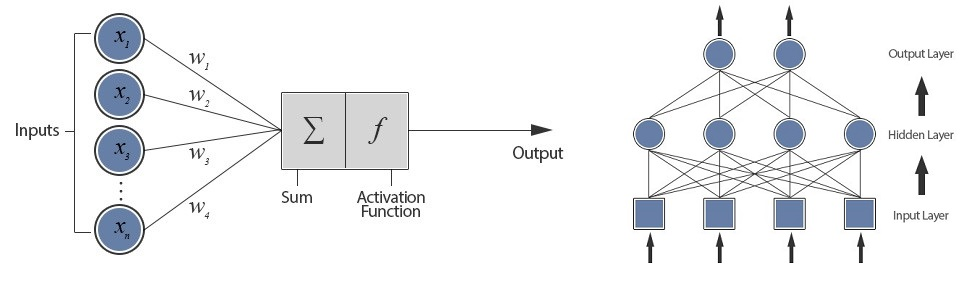
\includegraphics[width=\linewidth]{img/mix.jpeg}
  \caption{\small A perceptron and a neural network}
  \captionsource{\small Pokharna, Harsh. For Dummies — The Introduction to Neural Networks we all need ! (Parts 1 and 2) URL: https://medium.com/technologymadeeasy/for-dummies-the-introduction-to-neural-networks-we-all-need-c50f6012d5eb. Consulted: 24/4/2018}
  \label{fig:mix}
\end{figure}
 
 In the images in Figure \ref{fig:mix} we can see the basic structure of an ANN (artificial neural network). The left image depicts a node, the basic unit of the network. Each node performs a dot product between the input and weight values, that is, it takes the input values ($x_1... x_n$), multiplies each one by its respective weight ($w_1... w_n$) and sums everything up. The result of the dot product is passed to the activation function. If the result of this mathematical function is above a certain threshold, the node will fire and send an output value. In the right image can be seen a set of nodes structured in layers, with 4 in the input layer, 4 in the hidden layer and 2 in the output layer \cite{cs231n}. The input values are placed in the input nodes, which simply refer them to the nodes at the hidden layer. Each hidden node computes an output and forwards it to the output layer nodes, which make a final computation and generate a result \cite{airola2017}. Training the network consists of finding the best values for all the weights which optimize the results for most given cases. The presented example is very simplified, however, ANNs can have many different structures, with several hidden layers and other elements, such as a bias value \cite{cs231n}. \\


\subsection{Convolutional Neural Networks}
Convolutional neural networks are a specific kind of ANN usually used in computer vision and they usually take an image as an input. The general idea is that in each layer of the network the image is shrunken and processed by the activation functions in the neurons, and a new one is outputted which has partially abstracted any patterns found \cite{lee2009convolutional}. As the image goes from layer to layer, it becomes more abstract until it is finally tagged as belonging to some class. \\
Regular ANNs might work fine for small images, but do not scale well to bigger ones. "For example, an image of more respectable size, e.g. $200\times200\times3$ (3 stands for the RGB values of each pixel), would lead to neurons that have $200\times200\times3 = 120000$ weights. Moreover, we would almost certainly want to have several of such neurons, so the parameters would add up quickly. Clearly, this full connectivity is wasteful and the huge number of parameters would lead to overfitting." \cite{cs231n} \\
Since it is not computationally affordable to establish so many connections between nodes a new structure for the network has to be designed, with a new arrangement of the layers. Each layer has neurons disposed in 3 dimensions: width, height, and depth. Each neuron in a layer is only connected to a small group of neurons in the previous layer, which refers to adjacent pixels in the original image. What each layer does is to transform the 3D input volume to a 3D output volume of neuron activations \cite{cs231n}. [Figure \ref{fig:3DVolume}]

\begin{figure}[h!]
  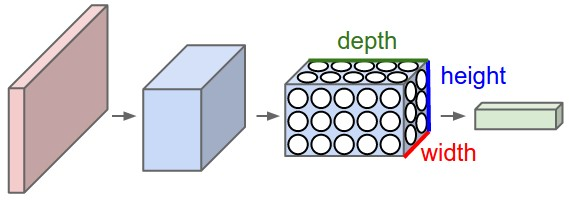
\includegraphics[width=\linewidth]{img/cnn.jpeg}
  \caption{\small A CNN transforms the 3D input volume from layer to layer.}
  \captionsource{\small Karpathy, Andrej. CS231n Convolutional Neural Networks for Visual Recognition \cite{cs231n}}
  \label{fig:3DVolume}
\end{figure}

\subsubsection{Types of layers}
\begin{outline}
	\1\textbf{Convolutional layers}: These layers are the principal building blocks of the CNN. The way they operate is by applying a set of filters to the input image trying to recognize patterns. These filters are quite smaller than the input image, (square matrices of $5\times5$ pixels, for example) so they have to slide or "convolve" from left to right and top to bottom along the whole image moving usually one pixel at a time (stride of 1). The dot product is computed between each filter and the portion of the image that is currently on focus, so the more similar they are to each other the higher the result will be and the greater influence it will have in the next layer's convolutions \cite{cs231n}. [Figure \ref{fig:convlayer}]
    \1\textbf{Pooling layers}: the function of the pooling layers is to gradually reduce the width and height of the input 3D volume as its depth keeps increasing due to the filtering process \cite{airola2017}. The most common pooling method is applying a filter of $2\times2$ pixels with a stride of 2 using the \textit{MAX} operation. This means that the image is divided into squared groups of 4 pixels and the maximum value of each group is taken, discarding the other three pixels, so its area is reduced by 3/4 \cite{cs231n}. [Figure \ref{fig:pooling}]
    \1\textbf{Fully connected layer}: All the nodes in the last layer have connections to all the activation inputs in the previous one. At this point, the image's dimensions have diminished and it has become small enough through the pooling process to feasibly compute a connection from each node to each pixel \cite{lee2009convolutional}. 
\end{outline}
\begin{figure}[h!]
  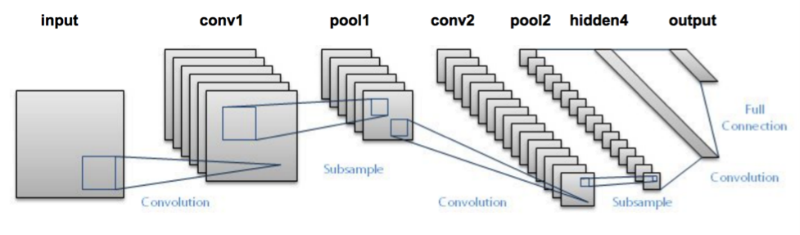
\includegraphics[width=\linewidth]{img/fullprocess.png}
  \caption{\small Filter sampling at convolutional layers}
  \captionsource{\small Dishashree, Gupta. Architecture of Convolutional Neural Networks (CNNs) demystified. URL: https://www.analyticsvidhya.com/blog/2017/06/architecture-of-convolutional-neural-networks-simplified-demystified/ Consulted: 27/5/2018}
  \label{fig:convlayer}
\end{figure}
\begin{figure}[h!]
  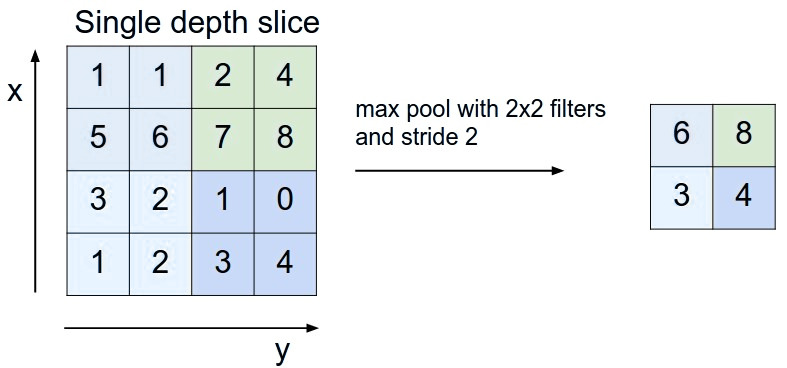
\includegraphics[width=\linewidth]{img/maxpool.jpg}
  \caption{\small \textit{MAX} operation usage at pooling layer.}
  \captionsource{\small Karpathy, Andrej. CS231n Convolutional Neural Networks for Visual Recognition \cite{cs231n}}
  \label{fig:pooling}
\end{figure}
 
\subsection{TensorFlow}
TensorFlow is a machine learning library developed by Google to satisfy their needs of systems capable of building and training neural networks \cite{tf_descpt}. Today it is used both for investigation purposes as well as in many of Google's own products. TensorFlow has been continuously expanding since its very beginnings. It was opensourced in 2015 and now the library is implemented in several programming languages and optimized for its use in different domains \cite{abadi2016tensorflow}. To run TensorFlow applications in mobile devices Google released first TensorFlow Mobile, which later evolved into TensorFlow Lite. These two frameworks are described and contrasted, since the main goal of the project is to compare their performance at the task of running CNNs.

\subsubsection{TensorFlow Mobile}
Running ANNs is a very computationally demanding task that has always been entrusted to powerful computers, but Google planned to take a step further and make the less powerful mobile devices capable of running them as well, since this would open a door with lots of potential. TensorFlow Mobile was developed to be able to run TensorFlow graphs on iOS and Android devices \cite{tfmobile}. When a TensorFlow graph is trained and ready for deployment it can be exported as a TensorFlow Mobile model with the protobuffer file format. A protobuffer is a file which contains all the relevant information about a graph \cite{varda2008protocol}. TensorFlow graphs are defined by their overall structure and the values of each of the weights. These two parts of the graph are usually stored in different files for convenience reasons, but they need to be put together in a protobuffer file to be used by TensorFlow Mobile on a mobile device. There are two types of protobuffer files: text format (\textit{file.pbtxt}) which is a human-readable form, and binary format (\textit{file.pb}) which is not readable but much smaller file \cite{tfmobile}. 

\subsubsection{TensorFlow Lite}
TensorFlow Lite is a natural evolution of TensorFlow Mobile, meant to substitute it in the long run. It was first released in November 2017, and it is still in a development stage \cite{tflite}. It presents many advantages over its predecessor: it generally provides better performance and a smaller binary file, but it does not cover all use cases yet. "TensorFlow Lite uses many techniques for achieving low latency such as optimizing the kernels for mobile apps, pre-fused activations, and quantized kernels that allow smaller and faster models" \cite{tflite}.
TensorFlow Lite's file format is the FlatBuffer (\textit{file.lite}), an "open-sourced, efficient cross-platform serialization library. It is similar to protocol buffers, but the primary difference is that FlatBuffers does not need an unpacking step to a secondary representation before you can access data, often coupled with per-object memory allocation." \cite{tflite}. It has also the capability of interacting with the Android Neural Networks API, designed specifically to boost machine learning computations \cite{zhang2018pcamp}. 

\subsection{Related work}
In the following section some examples of studies related to the topic of this thesis will be presented.

\subsubsection{Image Classification, Deep Learning and Convolutional Neural Networks}
In this comparative study of machine learning frameworks performed at Karlstad's university the authors analyse the performance for training netural networks in both TensorFlow and Microsoft CNTK, two machine learning frameworks available to the general public \cite{airola2017}. For the TensorFlow part, they chose tu use the third-party API Keras for specific tasks at the front-end. Their results are that CNTK performed better at the benchmarking tests, but TensorFlow with Keras is more intuitive and easy to work with. \\
This study is relevant since it gives some insights about other existing available frameworks for machine learning besides TensorFlow. Knowing about different posible setting up configurations for running neural networks can be useful for the present thesis.

\subsubsection{ImageNet Classification with Deep Convolutional Neural Networks}
The ImageNet classification paper by Alex Krizhevsky, Ilya Sutskever and Geoffrey E. Hinton represents one of the major breakthroughs in computer vision during 21st century. In 2012, a group of researchers designed deep convolutional neural network with five conv layers, some max pool layers and two globally connected layers \cite{alexnet}. The idea was to participate in the annual ImageNet Large-Scale Visual Recognition Challenge, where the participants present algorithms that have to classify input images over 1000 categories. With Alexnet (the name they gave to their CNN) they achieved  a top 5 test error rate of 15.4\%, considerably smaller than other solutions presented until that moment. This paper is relevant to the thesis since it suggest an efficient architecture to design CNNs.

\subsubsection{TensorFlow: A System for Large-Scale Machine Learning}
In this paper, the authors describe the TensorFlow dataflow model and demonstrate the compelling performance that TensorFlow achieves for several real-world applications \cite{abadi2016tensorflow}. The applicability of TensorFlow models to large scale systems requires a framework architecture which is optimal by every mean, since every single operation can become very computationally expensive in a large scale context. TPU (TensorFlow Processing Units) are presented with detail in the paper. They are a type of GPU specifically designed to train and execute neural networks, which saves enormous amounts of time in training graphs. This paper is relevant to the thesis since it informs about the possible approaches to handle massive inference requests for convolutional neural network systems.

\newpage
\section{Methodologies}\label{sec:method}
The upcoming chapter aims to describe the scientific and software development methods used for the realisation of this degree project. Some insight on the strategies followed to do research, as well as the methods selected to collect and analyse the data will be exposed. The software development methods chosen to create the deliverable are presented also.

\subsection{Research methods}
"Research methods and methodologies are processes, or particular courses of actions, that assure the quality of results of the research" \cite{haakansson}. As mentioned in the introductory chapter, their election is of a vital importance since it can affect the results and drewed conclusions of the research process. \\

The kind of research being done within this project is clearly quantitative since time is being measured, so its research method is "experimental". This research method is often used when investigating systems's performances \cite{haakansson}. The relative performance of two frameworks (TensorFlow Lite and TensorFlow Mobile) is being studied, and this one is determined by measuring the time taken for some computations to take place, which is a quantitative measurement. For this project, Positivism is chosen as the driving philosophical assumption, since it suits situations where a phenomenon needs to be probed in order to deepen in its understanding (such as in the present case).

\subsection{Research approaches}
The research approach chosen is mainly deductive. Deductive reasoning is the process of reaching a set of certain conclusions starting from a set of premises. If the premises are true and the logical rules are rigorously followed, then the arriving conclusions are necessarily true as well \cite{burns2000introduction}. A classical example of a deductive reasoning is the following:
\begin{center}
All men are mortal. (First premise) \\
Socrates is a man. (Second premise) \\
Therefore, Socrates is mortal. (Conclusion) \cite{dewey1914logical}\\
\end{center}
Deductive reasoning suits this research since by measuring how much time do the measurements take a logical conclusion can be drawn. An initial hypothesis is stated, TensorFlow Lite has a better performance in terms of time than its counterpart TensorFlow Mobile, since it has been developed to subsitute the latter. This theory needs to be severely tested using quantitative methods, and it will be accepted or discarded depending on the results of the tests. 

\subsection{Research design}
Selecting the correct research design or methodology to any study is an all-important task. This design will set the guidelines for organizing, planning, designing and conducting the research. The most common ones in quantitative studies are "ex post facto" research, experimental research, surveys and case studies. Furthermore, qualitative studies share as well some of these (surveys or case studies) but have as well some particular ones, such as action research, exploratory research, grounded theory and even etnography \cite{haakansson}. \\

After taking all research strategies into consideration, experimental research is opted as research design in this project. Experimental research concerns control over all factors that may affect the results of an experiment \cite{burns2000introduction}. As the research method, Experimental design verifies or falsifies hypotheses and provides cause-and-effect relationships between variables, i.e., correlations between independent and dependent variables \cite{haakansson}. In the present case there is control over the different factors that can influence the results of the experiment, namely the size of the image to be infered by the models, the device's operating system and its processor's computing power (the tests are performed in several devices with different characteristics). 
	
\subsection{Data collection}
The methods for data collection are the ones used to gather all the information that will be posteriorly analyzed and from which conclusions will be drew. Therefore it is vital to be able to guarantee precision and accuracy in the data collection, so that the results of the experiment are not biased. The most commonly used methods for quantitative research are experiments, questionnaire case study, and observation \cite{haakansson}. The chosen method for data collection is the experiment, a quantitative method used to gather samplings of large sets of variables. Experimental research often handles huge ammounts of data \cite{burns2000introduction}, so this method suited this thesis since many datapoints are collected. The order of magnitude of the dataset's size is adapted to the scope of the project. 150 measurements of time inference for each TensorFlow model are performed in each device, with images of three different pixel sizes (50 measurements each). Measuring the inference time of both models gives an idea of their real performance. Besides, it is worth mentioning that the interview, a qualitative method for data collection, is briefly used to collect the information about the requirements from the stakeholders.

\subsection{Data analysis}
The data analysis methods are used to analyse the collected material. It is the process of inspecting, cleaning, transforming and modelling data. It supports decision-making and drawing conclusions \cite{haakansson}. There exist several methods used for analysing quantitative data, such as statistics or computational mathematics. Statistics is the appropiate method to use in the present investigation since it summarizes the dataset into some values which are easier to work with \cite{burns2000introduction}. Parameters like the media or the standard desviation for each of the tests run will be calculated in order to have a degree of confidence in the conclusions drew.	

\subsection{Quality assurance}
Assuring the quality of an investigation means to validate and verify the research material. The quantiative research, with a deductive, approach, must apply and discuss validity, reliability, replicability and ethics \cite{haakansson} \cite{salkind} \cite{saunders}. \\

\subsubsection{Validity} \label{sssec:validity}
	The validity of the research confirms that the measurements are correct and accurate. As it will be later described, this validity is achieved by looking at the Android Profiler in Android Studio, a tool that lets us check the real execution time of each invoked function in an Android app. The measurement which is collected is the inference time for the CNN models to run, given exactly the same input. This measurement is done by setting timers in the device's processor through the Java API before and after the execution of the CNN, to calculate the time interval subsequently. These timers are accurate enough to make a realistic measure which lets a comparison between measurements be made.
\subsubsection{Reliability}
	Reliability means the stability of the measurements and the consistency of the results for every testing \cite{haakansson}. The repeated measurements obtained throughout this project are reliable since they remain moreless stable around fixed values (the variance is very low).
\subsubsection{Replicability}
	Replicability is the possibility of another researcher to replicate the experiment obtaining the same results. This is an important property of a project's methodology as it strengthens the integrity of the conclusions drawn in the research. The experiment is totally replicable, since the only things needed are a set of Android devices, installing the already implemented application on them and running the tests.
\subsubsection{Ethics and sustainability}
	Ethics and sustainability are the moral principles in planning, conducting and reporting results of research studies \cite{myers}. Ethics covers protection of participants, maintenance of privacy, avoiding coercion and having consent in written form, and treating material with confidentiality \cite{haakansson}. Sustainability extends to the consequences and impacts that the project might have on the enviroment and society.
	Ethics and sustainability in this project were introduced in section \ref{sssec:ethics}. The management the sensible information which can be found on credit card pictures (card number, owner's name, expiration date) should be taken into consideration. However, its is important to understand that this project never extracts the information on credit cards in a text format (it just generates a picture) and the credit card images used to train and test the network are computer generated.

\subsection{Software development methods}
There exist multiple software development methods for software project to effectively organize the work, implement all the requirements and reach the goals in time. All these methodological approaches can be classified in several types of models, like V-models, waterfall models or agile methods \cite{mccormick2012}, like Extreme Programming \cite{beck2000extreme} or Scrum \cite{schwaber2002agile}. Several methodological approaches were considered for the execution of this project. Some of them were discarded, like the waterfall or V-models, since they are designed to be used in large scale projects and take into consideration modifications of the requirements in the middle of the project. An important point to be taken into consideration is that only one person is in charge of this project, even if individuals from Slagkryssaren provided with counsil and help. This makes the whole development process much more flexible, since there is not a dependency of other people and work can be done at any place and at any time. For this reason, Scrum was chosen as software development method, because it has an agile approach, but it had to be adapted to a 1 person team \cite{schwaber2002agile}. Regarding the development enviroment and version control system, Android Studio together with Git were chosen.

\subsubsection{Scrum}
Scrum is an Agile framework for completing complex projects. Scrum originally was formalized for software development projects, but it works well for any complex, innovative scope of work \cite{alliance2016learn}. It is designed to break down the project into a set of actions which are iteratively run over through an specific time period, called sprint (very flexible, from 1 week to 1 month, but the duration remains constant along the project). The progress is tracked in short meetings scheduled at certain fixed moments along the day. These called daily scrums, and their purpose is to reflect upon the work done since the previous meeting and to readjust each participant's tasks and goals. In this way, what is important is always in mind and the team is aware of its performance \cite{rising2000scrum}. The participants of the project are called the Scrum team. In this team, several roles exist: the product owner, which represents the stakeholders and is in charge of assuring that all the requirements are fullfilled; the scrum master, which has the responsability of following the Scrum rules, and makes sure that there are no impediments or distractions which can affect the accomplishment of the goals. Finally, the development team, in charge of developing and delivering the potential product.

\subsubsection{Android and Android Studio IDE}
TensorFlow Mobile and TensorFlow Lite are available on two mobile platforms, iOS and Android. Android presents several advantages for the execution of this thesis and has been therefore chosen as host operative system \cite{developers2011android}. This advantages consist overall in the author's previous experience in the Android development framework, as well as the better integration capabilites that TensorFlow has with Android since they are both developed by Google. Some special functions such as the usage of the Neural Networks API were exclusively available on Android. The IDE chosen to develope the application with is Android Studio, which is built on JetBrains' IntelliJ IDEA software and designed specifically for developing Android applications \cite{studio2016official}.

\subsubsection{Git and Gitflow}
Git is the version control system used through out the project, together with the Gitflow workflow, being the repository with the code hosted in Bitbucket. 
Git tracks changes in the files stored in a given repository and coordinates the work done of them across teams of several people. It is most commonly used to track code files, but in practice it can be used to keep track of the changes in any kinds of files. Git allows to go back to individual milestones called commits, which present the different versions of the code. This commits do not necessarily follow a line in time, they can aswell divide in different branches with their own changes \cite{torvalds2010git}.
Gitflow is a workflow used with the Git version control system. It consists in a conventional set of rules for using Git in order to smooth and optimize the development process. It defines a branching model which focuses on product releases, with two principal branches: master (where the official released version of the program lies) and develop (where new functionality are implemented and tested). For each individual new feature a new branch is created which keeps the track of its development. When the new feature is ready it can be then merged back on to the develop branch, and when a set of new features are properly tested and seem to be working a new release is published in the master branch \cite{dwaraki2015gitflow}.
Using these version control tools was required by Slagkryssaren since they are the ones they use for all their other projects at the company.   

%\subsubsection{Design science}
%Design science is a problem solving approach which consists in presenting new artifacts into the enviroment. Artifacts are elements which contain knowledge, and they can widely include constructs, methods, models, design theories, etc \cite{von2004design}. There are 7 principal guidelines for design science research. First, design as an artifact which is produced; second, problem relevance (defining goals); third, design evaluation (the artifact's efficacy should be demonstrated);fourth, research contributions; fifth, research rigor; sixth, design as a search process and, finally, communication of research \cite{von2004design}.  These steps were implicitly followed to come up with the proposed method and evaluate its outcome.

% subsection subsection_name (end)
%Describe the engineering-related contents (preferably with models) and the research methodology and methods that are used in the degree project.

%\subsection{Engineering-related and scientific content:}
%Applying engineering-related and scientific skills; modeling, analyzing, developing, and evaluating engineering-related and scientific content; correct choice of methods based on problem formulation; consciousness of aspects relating to society and ethics (if applicable).

%As mentioned earlier, give a theoretical description of methodologies and methods and how these are applied in the degree project.
%Im unsure about what could I write here. I coul

\newpage
\section{Project design}
%\subsection{Literature study}
%The first natural step in the actual work was to familiarize myself with the theory and concepts behind CNNs as well as with the software tools I would be working with, namely TensorFlow. I spent quite some time reading about the functioning mechanism behind CNNs and also TensorFlow Mobile's and Lite's documentation. TensorFlow's documentation is quite extensive and at the same time is not specially unified, laying partially in GitHub and partially in their site. Often other portals such as Stack Overflow \cite{stackoverflow} or Medium.com were more useful and yielded working solutions to my problems. As well, I had to get acquainted with the current state of the project at Slagkryssaren, described in the following section. \\

In order to manage the project properly, the Scrum method was used, dividing the whole work in a series of 10 sprints, each of them lasting 9 days. For each sprint a set of goals were defined, usually including milestones that had to be surpassed in the development of the project. The first 8 sprints involved the main research and development of the application in the following way: 1 sprint invested in literature study and adaption to the new technologies, 1 sprint in exporting the TensorFlow models, 4 sprints in the development of the application and 1 sprint in testing the application in different devices and gathering the data. The last two sprints were used for writing this report. When a sprint came to an end, its results were evaluated and the tasks which had not been accomplished were posponed to the coming sprint.

\subsection{Project requirements}
At Slagkryssaren there is a research project, SKCC, which aims to build an API that receives pictures of credit cards and returns the data printed on them (i.e. the card number, expiry date, etc). To extract the information they use a convolutional neural network running in TensorFlow, but they are interested in making the API available for mobile devices, so the natural action is to reimplement the model with the mobile versions of TensorFlow. The recently launched framework TensorFlow Lite appears to be an attractive solution to them. \\

To understand which are the requirements demanded by Slagkryssaren, the interview is used as a data collection method. An interview with them was arranged, where they expressed their demands. The requirements consist in exporting the CNN to both TensorFlow Lite and TensorFlow Mobile file formats for later embedding them in an application which can compare their speed running tests. Another requirement is that such application is to be tested in different devices with different operating systems, in order to see how the performance of the two models varies. Images of different size should be fed into the system to see if the performance varies depending on this. Other requirements imposed by Slagkryssaren are that no part of the project's repository (including the dataset generator and other scripts) can be shared with third-party individuals alien to the company. Some software development requirements were stated as well: the version control system to keep track of the progress would be Git together with the Gitflow workflow, setting the parent repository in Bitbucket. \\  


\subsection{System architecture}
After stating the project's requirements pointed out by Slagkryssaren the system is ready to be designed in the form of an experiment (it is the research design chosen in the methodology). The system has several interconnected elements which can be seen in Figure \ref{fig:system}. First, the TensorFlow graph is exported in the two formats and compiled in an Android app using TensorFlow's APIs. Then, the credit card image generator already implemented by Slagkryssaren is used to create a set of new images, and these are fed to the two versions of the graph. The inference time taken by each of them to produce an output is measured and stored in the device. To achieve reliability in the measurements the sets of images had to be big enough, and of different sizes to check how the input size affected the performance of the models (see requirements above). Three sets of 50 images, with dimensions $ 160\times160 $, $ 240\times240 $, and $ 320\times320 $ pixels would be generated for this purpose. Other variables to be considered are the device's computational power and the operating system being run on it. For this purpose, four devices which represent different areas of these variable's spectrum were selected for running the experiment, namely a Samsung Galaxy S8 (Android 8.0), a Samsung Galaxy S5 (Android 5.0.1), a Samsung Galaxy S4 (Android 4.4.2) and a Motorola Moto G5 Plus (Android 7.0). 
\begin{figure}[h!]
  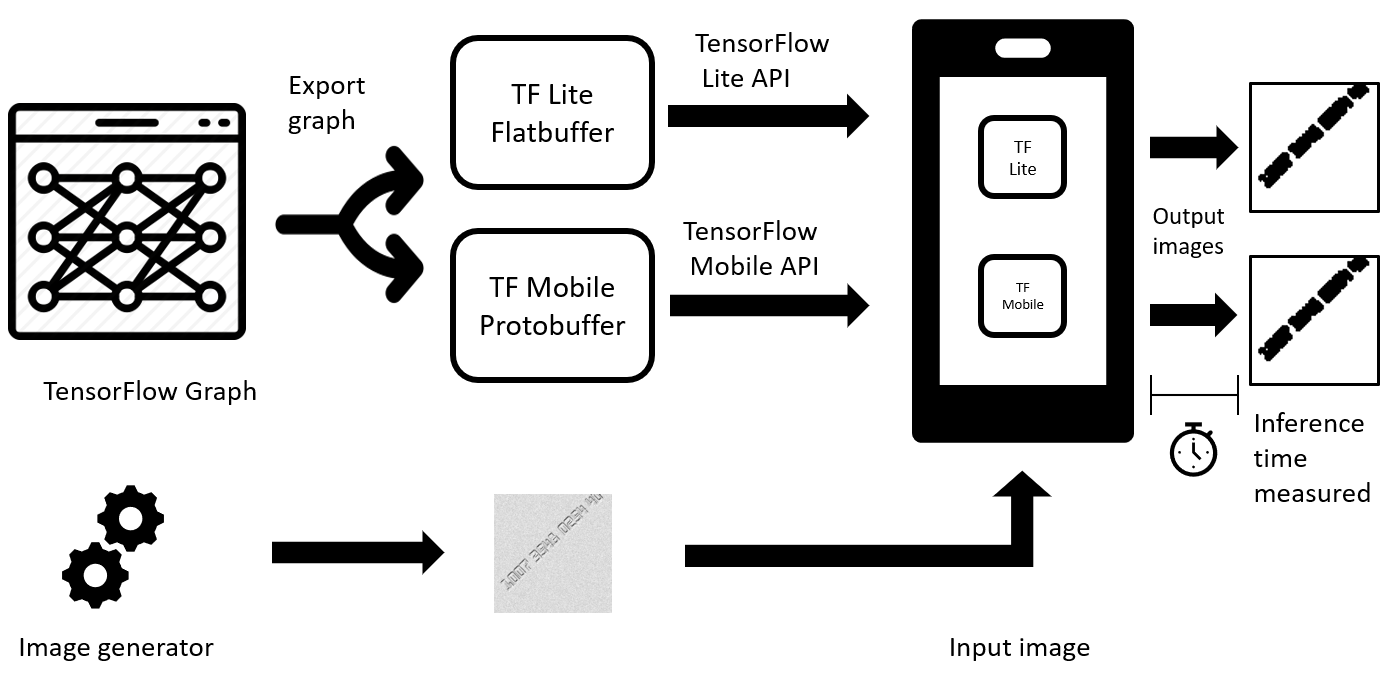
\includegraphics[width=\linewidth]{img/system.png}
  \caption{\small System architecture}
  \captionsource{\small The TensorFlow Graph picture inside the diagram is obtained from https://d30y9cdsu7xlg0.cloudfront.net/png/1705433-200.png}
  \label{fig:system}
\end{figure}

\subsection{Initial state of the project}
The project in which Slagkryssaren is working on consists, as aforementioned in the introduction, in developing a TensorFlow graph which could analyze a picture of a credit card and return the information printed on it. This project started in June 2016 but not many resources were invested into it, so it is still in an early phase when first shared with me. 
The TensorFlow graph which they had written at the time consists in a CNN which removes the background noise and returns a black and white image where only the credit card number can be seen. To create a dataset to train this graph they programmed the credit card image generator which produces fairly realistic pictures. Figure \ref{fig:removeback} is an example of one of the thousands of pairs of images generated to train the network. The left image is fed into the input and the right image is the target, that is, what the network is expected to produce. The graph had been trained on them and the results were satisfying. \\
%Attach picture of CNN from TensorBoard.
%\begin{wrapfigure}{r}{9cm}
%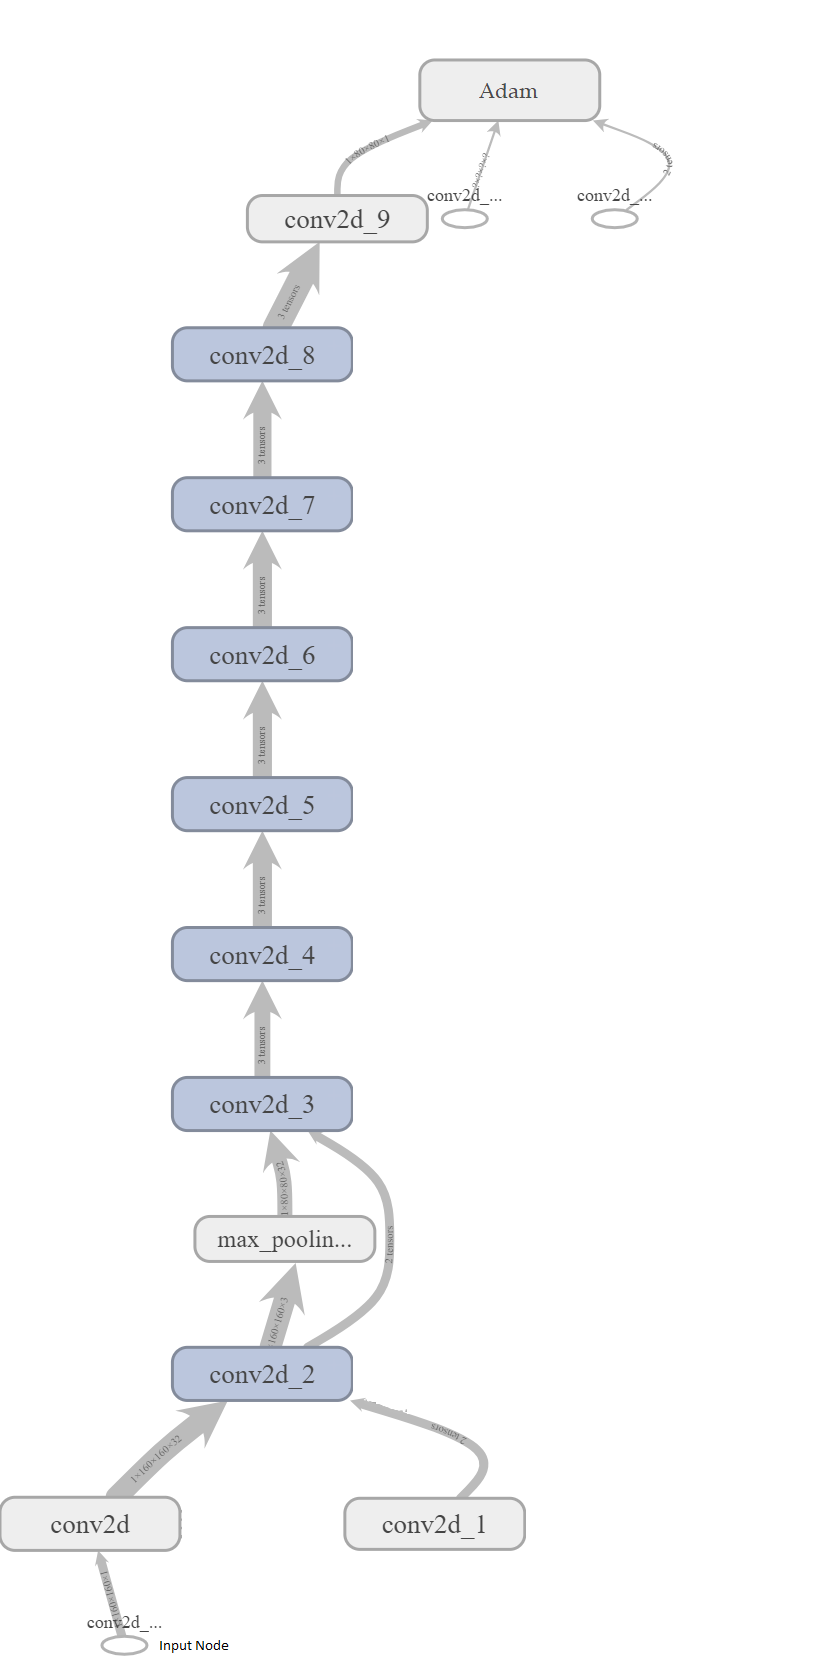
\includegraphics[width=9cm]{img/Tensorboard.png}
%\caption{\small Graph of the CNN used on the credit card images}\label{fig:tensorboard}
%\vspace{-10pt}
%\end{wrapfigure} 
\begin{figure}[h]
\centering
  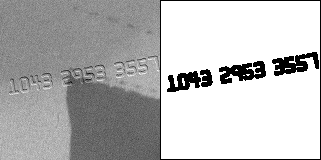
\includegraphics[width=9.0cm]{img/img_target.png}
  \caption{\small Example of input (left) and target (right) images used to train the CNN.}
  \captionsource{\small Images produced with the credit card image generator developed at Slagkryssaren}
  \label{fig:removeback}
\end{figure}


Figure \ref{fig:tensorboard} reveals the inner structure of the CNN. \textit{Conv2d} is the input layer, backed by \textit{Conv2d\_1} which adds a bias, then it comes a convolutional layer \textit{Conv2d\_2}, followed by a MAX pooling layer with a stride of 2 and a filter of 2x2 pixels. The image is now reduced to a quarter of its size. Afterwards, it goes through 6 more convolutional layers (\textit{Conv2d\_3}to \textit{Conv2d\_8} both included) with a stride of 1 and a filter of 5x5. Convolutional layers \textit{Conv2d\_2-8} use \textit{relu} as activation function. In the last convolutional layer \textit{Conv2d\_9} the filter is changed to 1x1 and activation function to a \textit{sigmoid}. The data is then sent to the Adam module which performs some optimizations which are beyond the scope of this thesis. The network has not a fully connected layer in the end, though, since the output of the graph is not yet meant to make a classification, but still generates a picture. All these values were chosen for the configuration of the network since they are optimal standard values in CNN architectures \cite{cs231n}. In some of the arrows which connect the different layers can be appreciated the size of the 4-dimensional float vector which represents the image. In other arrows, the number of tensors between layers is pointed out. This convolutional network developed by Slagkryssaren was adequate for studying the performance of the TensorFlow frameworks for mobile devices, so it was selected. \\

\begin{figure}[p!]
\centering
  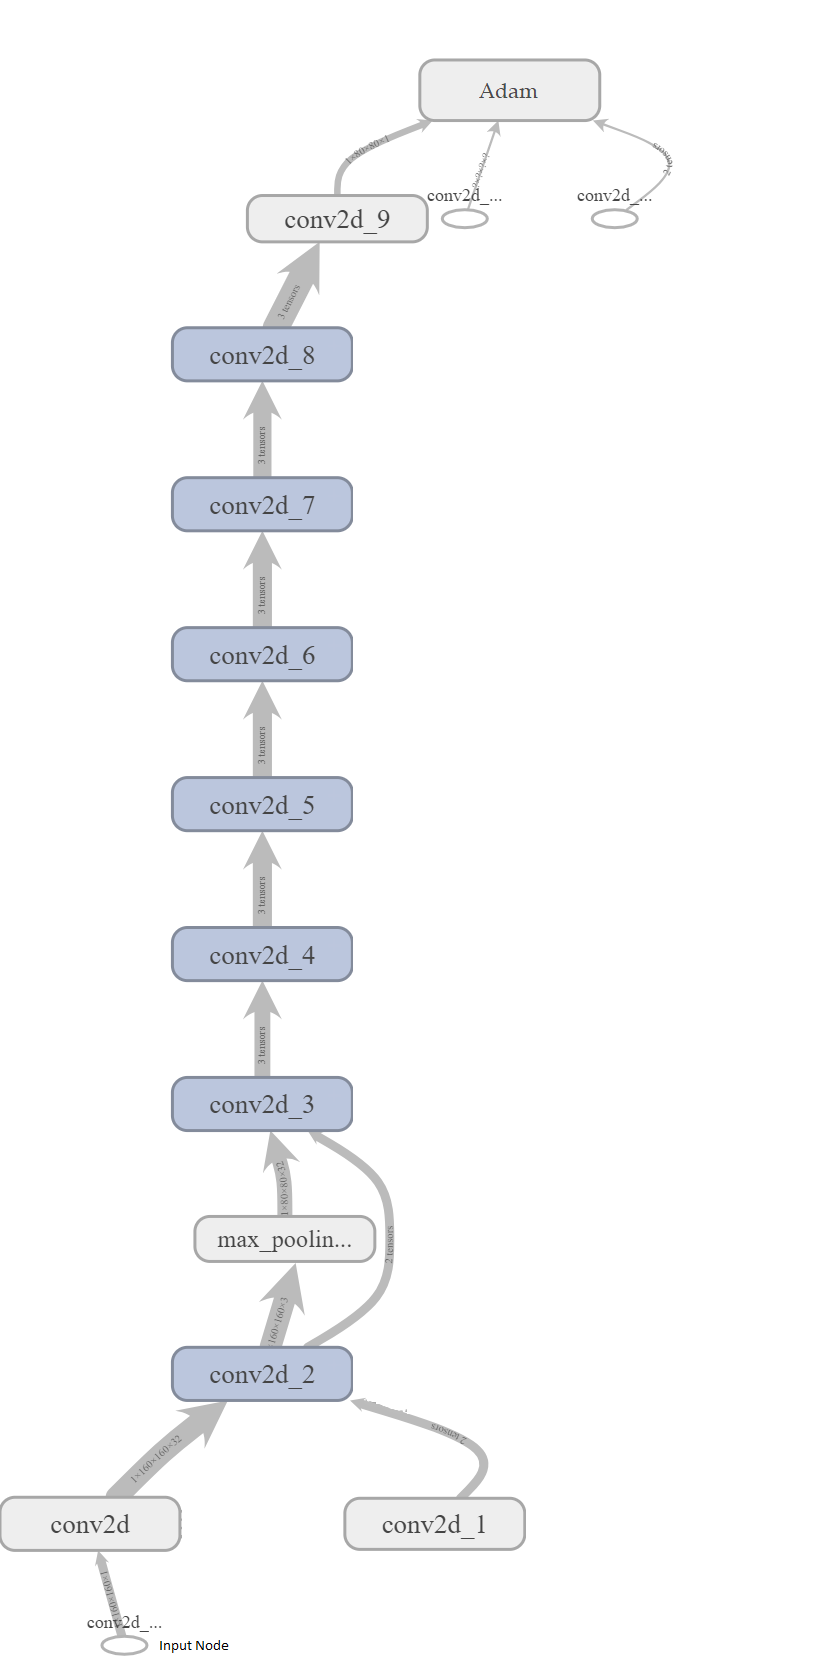
\includegraphics[width=0.8\textwidth]{img/Tensorboard.png}
  \caption{\small Graph of the CNN used on the credit card images}
  \captionsource{\small Exported from TensorBoard}
  \label{fig:tensorboard}
\end{figure}

In this chapter the project requirements have been stated, together with the designed architecture of the system which fullfills all of them. The initial state of the project "as is" is presented as well. \\

\newpage
\section{Implementation of the test application}
The implementation of the test application consists of several steps. The first one is to export the graph from the TensorFlow framework in the computer as both TensorFlow Mobile and TensorFlow Lite models. The second is to develop the Android application which would iteratively feed the generated pictures into the models and register their inference time. These two steps are described in the following sections, whereas the final stage of testing it in the set of devices will be explained later on. 

\subsection{Exporting the graph}
After the research was done it was time to export the CNN as both a TensorFlow Mobile model and a TensorFlow Lite model to be able to use them in an Android application. The graph had to be "frozen" first, that is, all the variable values for the weights had to be converted into inline constants \cite{TFdeploy}. The function \textit{freeze\_session()} contained in \textit{freeze\_graph.py} in the TensorFlow library allows us to do this. Then it is time to write the frozen graph into a file, and this will be done in different ways depending on the TensorFlow version which is going to run it and on the output format desired for the file. \\

To get a model runnable by TensorFlow Mobile there were different possible output formats for the file, but the raw protobuffer format (with extension \textit{.pb}) was preferred. The function \textit{write\_graph()} is invoked, specifying the path and the output format of the model, and it generates a file. For the TensorFlow Lite model, the process followed is slightly different, since there is an intermediate step between freezing and writing the graph to a file. The frozen graph has to be converted first to a TensorFlow Lite graph using TOCO (TensorFlow Lite Optimizing Converter). This is done by invoking the function \textit{toco\_convert()}. The resulting graph is then written to a file with flatbuffer format (\textit{.lite}). \\

\subsection{Development of testing application}
Once the two models had been retrieved the development of a test application could start. The application's purpose is to be able to quickly test the relative performance of both models by running them over a set of images on different devices. The time it takes to run the models for each image is stored and displayed in a nice graph to get an overview of the performance of each model. All this inference data can be easily exported from the app to a text file for posterior analysis. The development of the Android application took a considerable portion of the work time used for this project. My personal experience with the Android environment was somehow limited, and the TensorFlow Lite and Mobile dependency libraries for Android were totally new to me. TensorFlow Lite 0.1.7 and TensorFlow Mobile 1.8.0 are the versions used in this project.
The app was divided into different activities: \\
\begin{outline}
\1\textbf{MainActivity}: runs the models and displays a grid with the pictures to be analyzed. When any of the pictures are clicked, the models are run on that picture and the result is displayed in DisplayActivity. [Figure \ref{fig:MainActivity}]. 
\1\textbf{DisplayActivity}: after running the models it plots the picture, the target (expected result), and both of the predictions of the TFLite and TFMobile models, together with their respective inference times. [Figure \ref{fig:DisplayActivity}]
\1\textbf{StatsActivity}: plots a chart where it is represented the inference run time of both models for each picture. Each time a model is run on a picture, a new point is added to the chart. [Figure \ref{fig:StatsActivity}]
\1\textbf{SettingsActivity}: used to configure the settings for the test, such as the number of images selected to run the model on, which model or models to use and the usage of the Neural Networks API if available. The data on the chart can be exported from here to a text file (Export button), or totally erased as well (Erase button). [Figure \ref{fig:SettingsActivity}]
\1\textbf{CameraActivity}: lets the user take a picture with the device camera and run the models on it.
\end{outline}
A parent Model class has been also implemented with some abstract methods, from which specific TfLiteModel and TfMobileModel classes are extended. An Adapter class for the picture grid and a BaseActivity have been implemented as well.
%Development of testing application: Design of the app: library of images, settings view, chart view. The app runs the two models (TensorFlow Lite and TensorFlow Mobile) iteratively over a set of images, and plots the inference time of the two models in a chart. One can export the collected data to a file afterwards. 
\begin{figure}[]
	\centering 
	\begin{subfigure}[p]{0.45\textwidth}
	  \centering
	  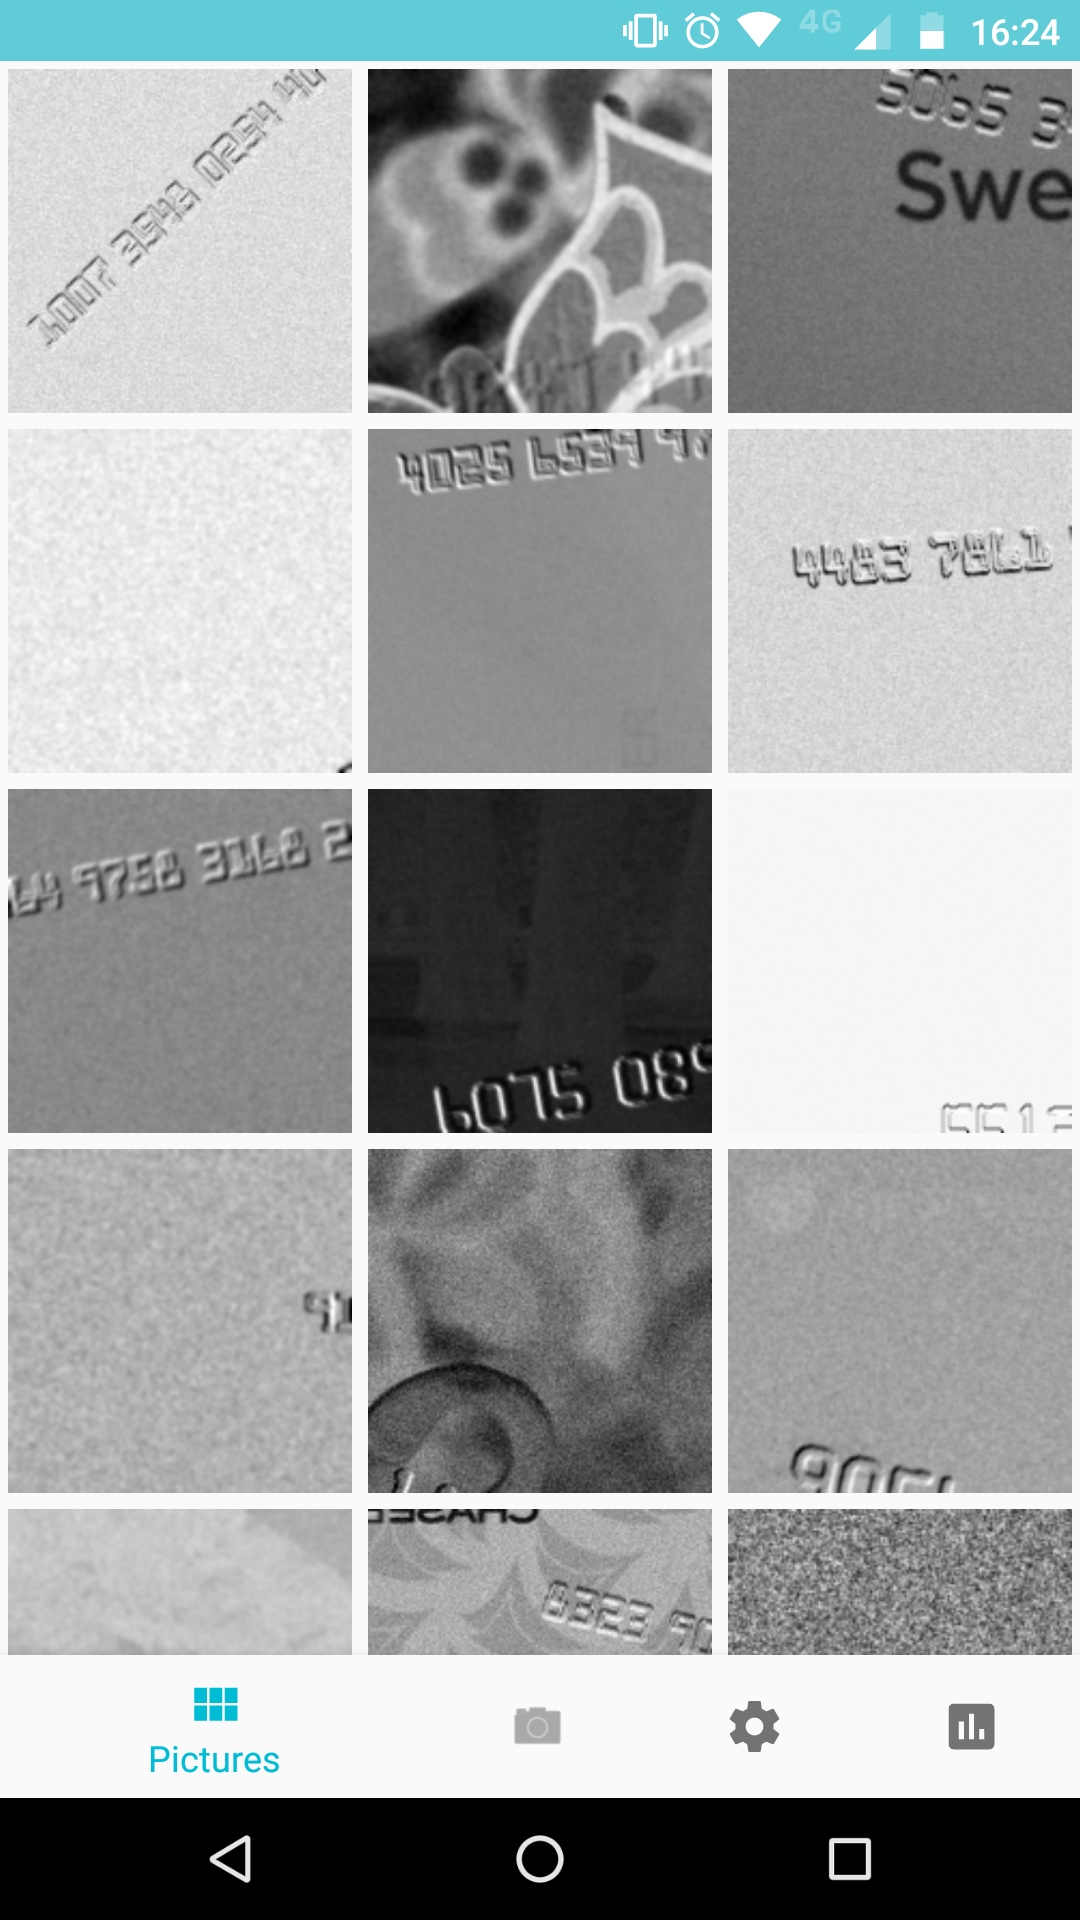
\includegraphics[width=0.75\textwidth]{img/app/main.png}
	  \captionof{figure}{\footnotesize MainActivity: presents a grid with pictures which will be run on the models when clicked.}
	  \label{fig:MainActivity}
	\end{subfigure}
	\quad
	\begin{subfigure}[p]{0.45\textwidth}
	  \centering
	  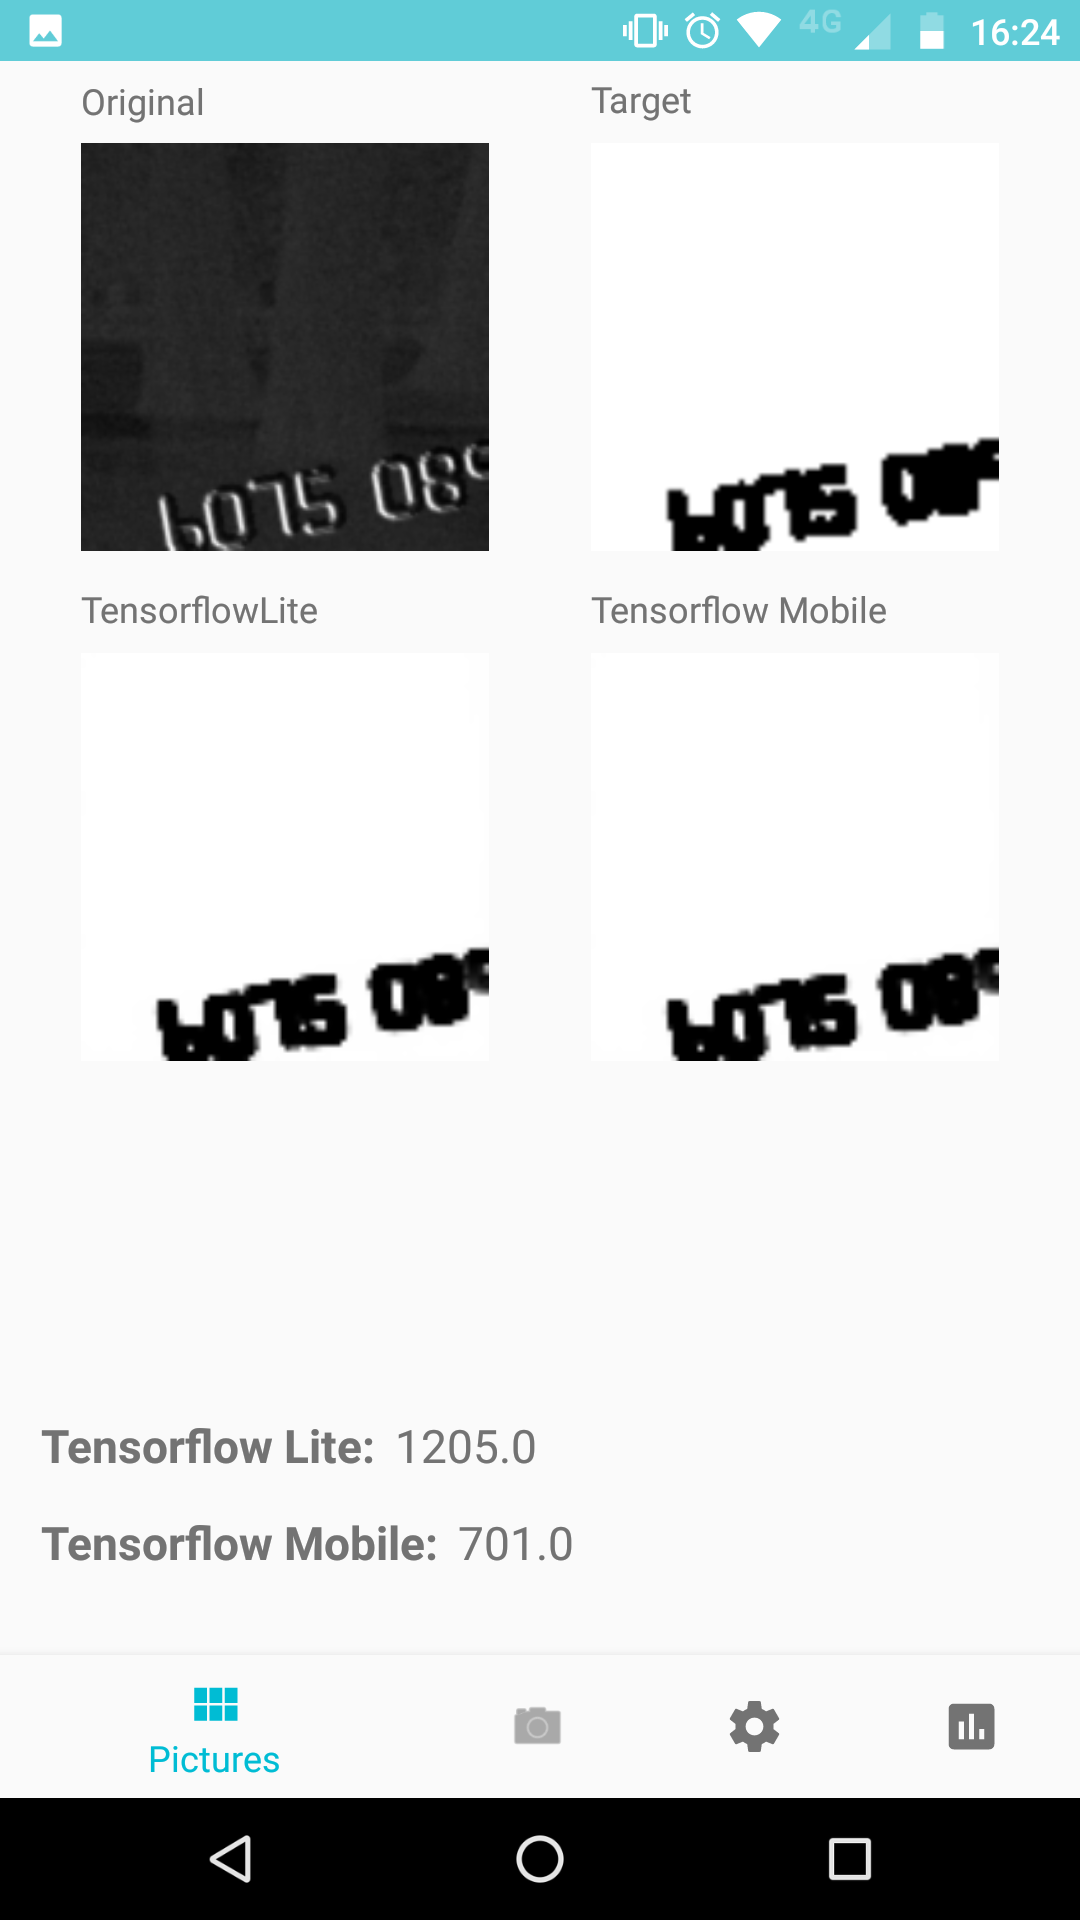
\includegraphics[width=0.75\textwidth]{img/app/display.png}
	  \captionof{figure}{\footnotesize DisplayActivity: after running the model displays the input picture, the target and the predictions of the models with their inference times.}
	  \label{fig:DisplayActivity}
	\end{subfigure}
	\newline
	\vskip\baselineskip
	\begin{subfigure}[p]{0.45\textwidth}
	  \centering
	  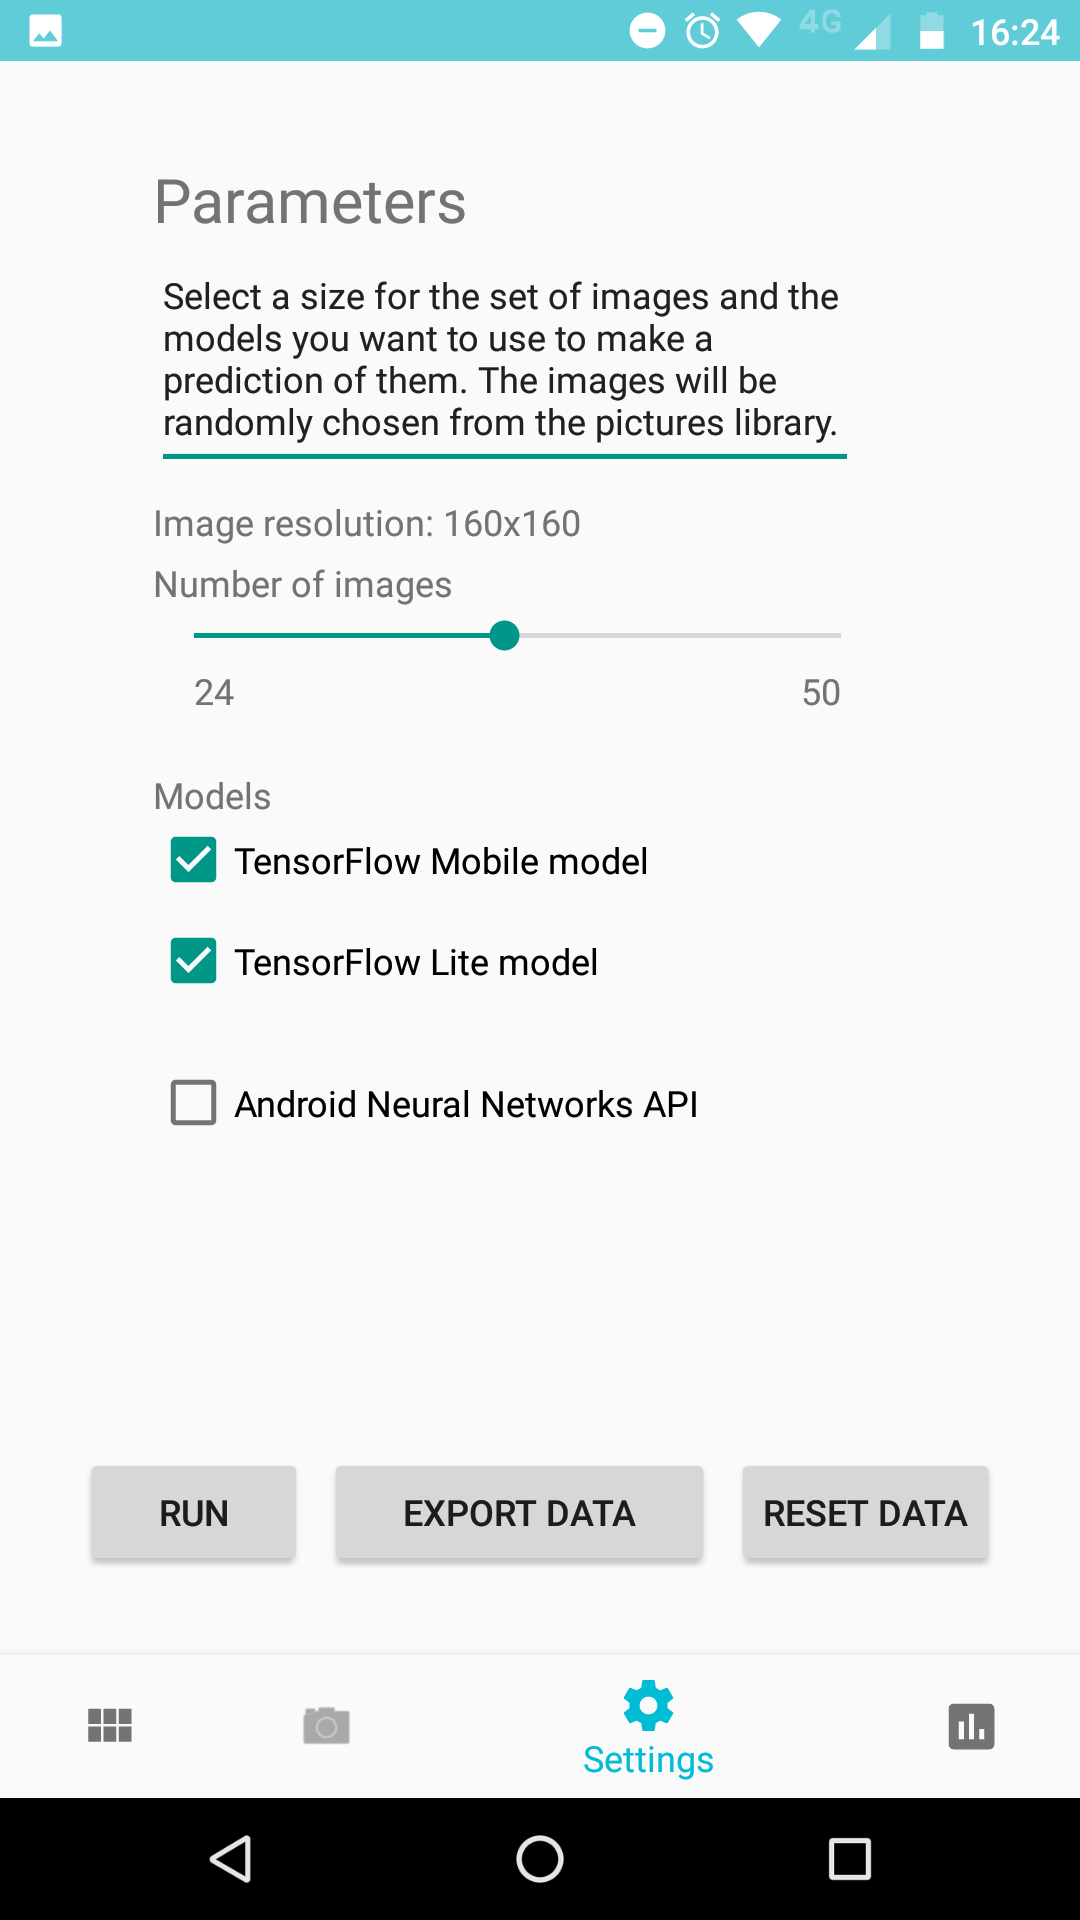
\includegraphics[width=0.75\textwidth]{img/app/settings.png}
	  \captionof{figure}{\footnotesize SettingsActivity: Menu to run the models on multiple images (number selected with the slider). The collected data points can be written to a file (export button) or erased (reset button).}
	  \label{fig:SettingsActivity}
	\end{subfigure}
	\quad
	\begin{subfigure}[p]{0.45\textwidth}
	  \centering
	  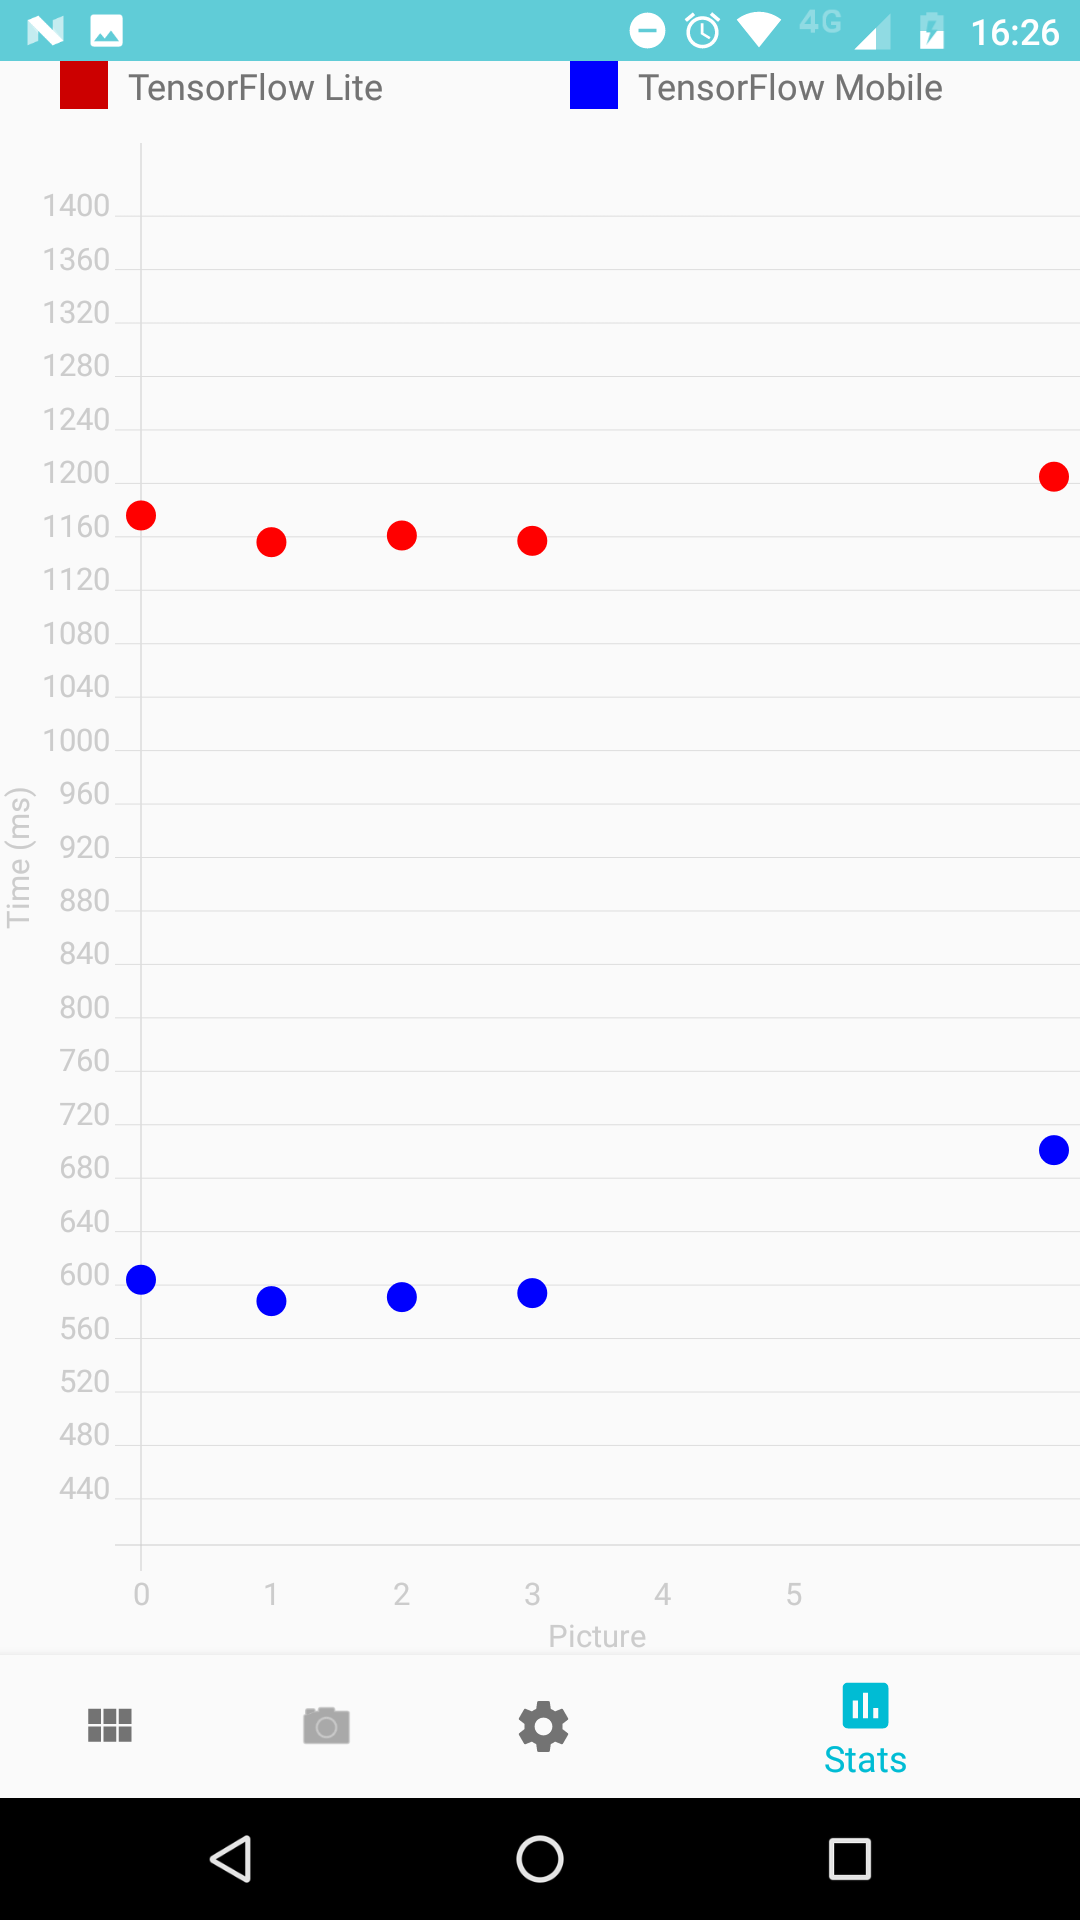
\includegraphics[width=0.75\textwidth]{img/app/stats.png}
	  \captionof{figure}{\footnotesize StatsActivity: displays a chart which compares the inference time between the two models for each image.}
	  \label{fig:StatsActivity}
	\end{subfigure}
	\caption[] {\footnotesize Principal activities in test application}
	\label{fig:Activities}
\end{figure}
TfMobileModel and TfLiteModel classes have similar implementations of the \textit{predictImage()} method, which is used to actually run the model on an image. This function converts the image in Bitmap format to a float array, starts then a time counter, feeds the float array to the model, stops the timer when the computation has finalized and reconstructs a Bitmap image from the output float array. Both implementations follow. \\
%\newpage
\begin{lstlisting}[language = Java, basicstyle=\scriptsize,caption={\small code in \textit{predictImage()} used for TfMobileModel}\label{lst:codeTfMobile}]
inputData = convertBitmapToFloatArray(bitmap);
long startTime = SystemClock.uptimeMillis();
infInterface.feed(inputName, (float[]) inputData, 1, IMAGE_DIM_X, IMAGE_DIM_Y, 1);
infInterface.run(new String[]{outputName}, true);
infInterface.fetch(outputName, (float[]) outputData);
long endTime = SystemClock.uptimeMillis();
Bitmap outputImage = convertFloatArrayToBitmap(outputData);
\end{lstlisting}

\begin{lstlisting}[language = Java, basicstyle=\scriptsize,caption={\small code in \textit{predictImage()} used for TfLiteModel}\label{lst:codeTfLite}]
inputData = convertBitmapToFloatArray(bitmap);
tflite.setUseNNAPI(neuralAPI);
long startTime = SystemClock.uptimeMillis();
tflite.run(inputData, outputData);
long endTime = SystemClock.uptimeMillis();
Bitmap outputImage = convertFloatArrayToBitmap(outputData);
\end{lstlisting}

The principal difference between both approaches is that the TensorFlow Lite execution of the model (listing \ref{lst:codeTfLite}) is atomical and happens within one function call while TensorFlow Mobile (listing \ref{lst:codeTfMobile}) subdivides the whole operation in feeding the model with data, running it, and fetching the results. The input vector differs between both implementations, being a one dimensional float array (float[]) for TensorFlow Mobile and a four-dimensional float array (float [][][][]) for TensorFlow Lite.
When the Android application was completed and fully operational several tests were run in a handful of devices. The results of these tests are described in the following section. \\


The process followed to implement the system  has been thoroughly described, first explaining the export of the model in to the two different file formats and then illustrating the inner architecture of the Android application. The upcoming section presents the testing. \\

\newpage
\section{Test execution}
When the application development phase was satisfactorily completed the project could carry on with the test phase. The application was exported from Android Studio (the IDE platform used to program it) as an apk file, the standard Android application package format, and installed on the selected devices. The tests were executed according to the design and the measured data was exported. Tables \ref{table:S8}-\ref{table:G5} present several statistical numerals about the inference times of the three different sets of images in each device, namely the average time of all images in a set $\overline{x}$, the standard deviation $\sigma$ and the relative standard deviation \textit{RSD}. Figures \ref{fig:S8}-\ref{fig:G5} display in a graph the values of the average inference times, to give the reader an intuitive impression of their relative magnitudes. The information contained in these tables and figures helps to arrive to some conclusions later on.\\

\subsection{Test 1: Samsung Galaxy S8}
The Samsung Galaxy S8 performed very well in the test. This does not surprise since it is Samsung's flagship device for the year 2017 and by far the most powerful of all the devices being tested. The relative standard deviation is very low for the different sets of images, so the measurements do not vary much. Table \ref{table:S8} and Figure \ref{fig:S8} reflect the resulted values of processing the collected data with statistics, the data analysis tool selected in the methodology. \\

\begin{table}[h!]
\centering
\resizebox{\textwidth}{!}{%
\begin{tabular}{@{}rcrlrrl@{}}
\toprule
\multicolumn{1}{l}{\textbf{Samsung Galaxy S8}} & \multicolumn{3}{l}{\textbf{TF Mobile}} & \multicolumn{3}{l}{\textbf{TensorFlow Lite}} \\ \midrule
\multicolumn{1}{|l|}{} & \multicolumn{1}{l}{\textit{$\overline{x}$ (ms)}} & \multicolumn{1}{l}{\textit{$\sigma$ (ms)}} & \multicolumn{1}{l|}{\textit{RSD $\sigma$/ $\overline{x}$ (\%)}} & \multicolumn{1}{l}{\textit{$\overline{x}$ (ms)}} & \multicolumn{1}{l}{\textit{$\sigma$ (ms)}} & \multicolumn{1}{l|}{\textit{RSD $\sigma$/ $\overline{x}$ (\%)}} \\ \cmidrule(l){2-7} 
\multicolumn{1}{|r|}{\textbf{160x160 px}} & \multicolumn{1}{c|}{\textit{182,44}} & \multicolumn{1}{r|}{5,8} & \multicolumn{1}{l|}{3,2} & \multicolumn{1}{r|}{371,52} & \multicolumn{1}{r|}{24,3} & \multicolumn{1}{l|}{6,5} \\ \cmidrule(l){2-7} 
\multicolumn{1}{|r|}{\textbf{240x240 px}} & \multicolumn{1}{c|}{\textit{410,12}} & \multicolumn{1}{r|}{12,7} & \multicolumn{1}{l|}{3,1} & \multicolumn{1}{r|}{814,16} & \multicolumn{1}{r|}{30,3} & \multicolumn{1}{l|}{3,7} \\ \cmidrule(l){2-7} 
\multicolumn{1}{|r|}{\textbf{320x320 px}} & \multicolumn{1}{c|}{\textit{757,34}} & \multicolumn{1}{r|}{19,4} & \multicolumn{1}{l|}{2,6} & \multicolumn{1}{r|}{1494,28} & \multicolumn{1}{r|}{49,9} & \multicolumn{1}{l|}{3,3} \\ \bottomrule
\end{tabular}%
}
\caption{Samsung Galaxy S8 test results}
\label{table:S8}
\end{table}

\begin{figure}[p]
  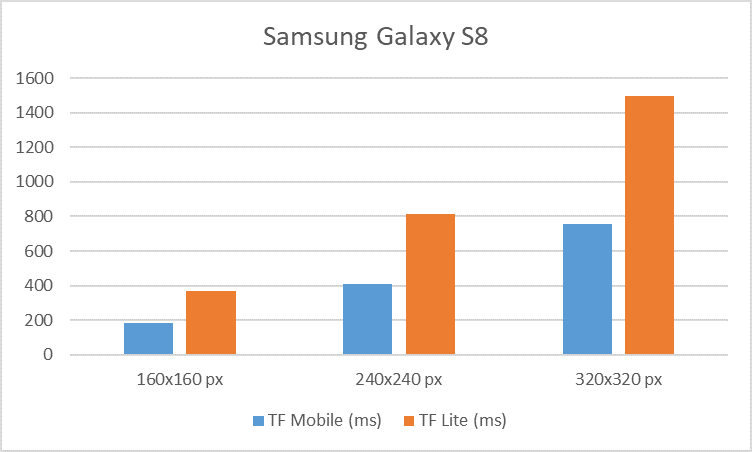
\includegraphics[width=\linewidth]{img/charts/S8.png}
  \captionof{figure}{\small Samsung Galaxy S8 average inference times. This figure reflects the data from table \ref{table:S8}}
  \label{fig:S8}
\end{figure}

\subsection{Test 2: Samsung Galaxy S5}
The Samsung Galaxy S5 is also a powerful device, and it headed the top line of Samsung smartphones in its time, but now it is getting outdated and we can see that its performance is not as good as the S8. It runs an older version of the Android OS (4.4), even though a new one is available for this model. Still, the relative standard deviation is low as well. Table \ref{table:S5} and Figure \ref{fig:S5} reflect the resulted values of processing the collected data with statistics, the data analysis tool selected in the methodology. \\

\begin{table}[h!]
\centering
\resizebox{\textwidth}{!}{%
\begin{tabular}{@{}rcrlrrl@{}}
\toprule
\multicolumn{1}{l}{\textbf{Samsung Galaxy S5}} & \multicolumn{3}{l}{\textbf{TF Mobile}} & \multicolumn{3}{l}{\textbf{TensorFlow Lite}} \\ \midrule
\multicolumn{1}{|l|}{} & \multicolumn{1}{l}{\textit{$\overline{x}$ (ms)}} & \multicolumn{1}{l}{\textit{$\sigma$ (ms)}} & \multicolumn{1}{l|}{\textit{RSD $\sigma$/ $\overline{x}$ (\%)}} & \multicolumn{1}{l}{\textit{$\overline{x}$ (ms)}} & \multicolumn{1}{l}{\textit{$\sigma$ (ms)}} & \multicolumn{1}{l|}{\textit{RSD $\sigma$/ $\overline{x}$ (\%)}} \\ \cmidrule(l){2-7} 
\multicolumn{1}{|r|}{\textbf{160x160 px}} & \multicolumn{1}{c|}{462,9} & \multicolumn{1}{r|}{25,7} & \multicolumn{1}{l|}{5,6} & \multicolumn{1}{r|}{1006,38} & \multicolumn{1}{r|}{69,3} & \multicolumn{1}{l|}{6,9} \\ \cmidrule(l){2-7} 
\multicolumn{1}{|r|}{\textbf{240x240 px}} & \multicolumn{1}{c|}{931,6} & \multicolumn{1}{r|}{42,6} & \multicolumn{1}{l|}{4,6} & \multicolumn{1}{r|}{2212,34} & \multicolumn{1}{r|}{79,7} & \multicolumn{1}{l|}{3,6} \\ \cmidrule(l){2-7} 
\multicolumn{1}{|r|}{\textbf{320x320 px}} & \multicolumn{1}{c|}{2587,76} & \multicolumn{1}{r|}{105,3} & \multicolumn{1}{l|}{4,1} & \multicolumn{1}{r|}{5777,78} & \multicolumn{1}{r|}{215,8} & \multicolumn{1}{l|}{3,7} \\ \bottomrule
\end{tabular}%
}
\caption{Samsung Galaxy S5 test results}
\label{table:S5}
\end{table}

\begin{figure}[p]
  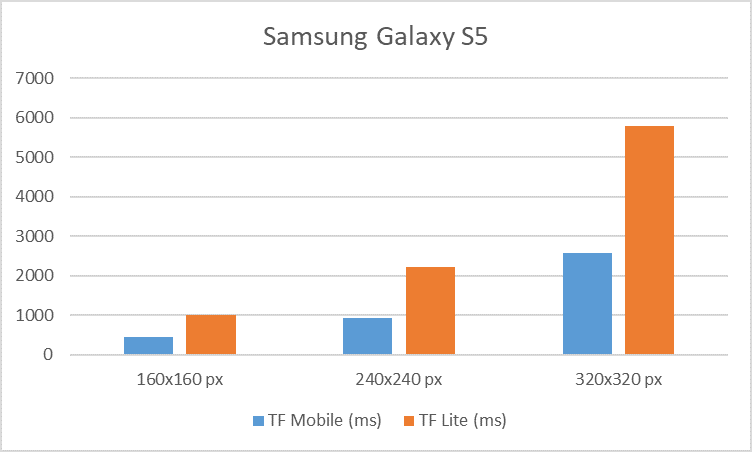
\includegraphics[width=\linewidth]{img/charts/S5.png}
  \captionof{figure}{\small Samsung Galaxy S5 average inference times. This figure reflects the data from table \ref{table:S5}}
  \label{fig:S5}
\end{figure}

\subsection{Test 3: Samsung Galaxy S4}
For today's standards, the Samsung Galaxy S4 is an average phone. We see that the performance of both models clearly drops with this device, especially with the bigger images. The relative standard deviation increases with the image size up to 17\%. The slightly more modern version of the OS (5.0.2) does not help in improving the results. Table \ref{table:S4} and Figure \ref{fig:S4} reflect the resulted values of processing the collected data with statistics, the data analysis tool selected in the methodology. \\

\begin{table}[h!]
\centering
\resizebox{\textwidth}{!}{%
\begin{tabular}{@{}rcrlrrl@{}}
\toprule
\multicolumn{1}{l}{\textbf{Samsung Galaxy S4}} & \multicolumn{3}{l}{\textbf{TF Mobile}} & \multicolumn{3}{l}{\textbf{TensorFlow Lite}} \\ \midrule
\multicolumn{1}{|l|}{} & \multicolumn{1}{l}{\textit{$\overline{x}$ (ms)}} & \multicolumn{1}{l}{\textit{$\sigma$ (ms)}} & \multicolumn{1}{l|}{\textit{RSD $\sigma$/ $\overline{x}$ (\%)}} & \multicolumn{1}{l}{\textit{$\overline{x}$ (ms)}} & \multicolumn{1}{l}{\textit{$\sigma$ (ms)}} & \multicolumn{1}{l|}{\textit{RSD $\sigma$/ $\overline{x}$ (\%)}} \\ \cmidrule(l){2-7} 
\multicolumn{1}{|r|}{\textbf{160x160 px}} & \multicolumn{1}{c|}{516,9} & \multicolumn{1}{r|}{43,8} & \multicolumn{1}{l|}{8,5} & \multicolumn{1}{r|}{1397,58} & \multicolumn{1}{r|}{135,1} & \multicolumn{1}{l|}{9,7} \\ \cmidrule(l){2-7} 
\multicolumn{1}{|r|}{\textbf{240x240 px}} & \multicolumn{1}{c|}{1307,1} & \multicolumn{1}{r|}{160,9} & \multicolumn{1}{l|}{12,3} & \multicolumn{1}{r|}{3562,82} & \multicolumn{1}{r|}{428,7} & \multicolumn{1}{l|}{12,0} \\ \cmidrule(l){2-7} 
\multicolumn{1}{|r|}{\textbf{320x320 px}} & \multicolumn{1}{c|}{3360,74} & \multicolumn{1}{r|}{571,8} & \multicolumn{1}{l|}{17,0} & \multicolumn{1}{r|}{9679,18} & \multicolumn{1}{r|}{1663,7} & \multicolumn{1}{l|}{17,2} \\ \bottomrule
\end{tabular}%
}
\caption{Samsung Galaxy S4 test results}
\label{table:S4}
\end{table}

\begin{figure}[p]
  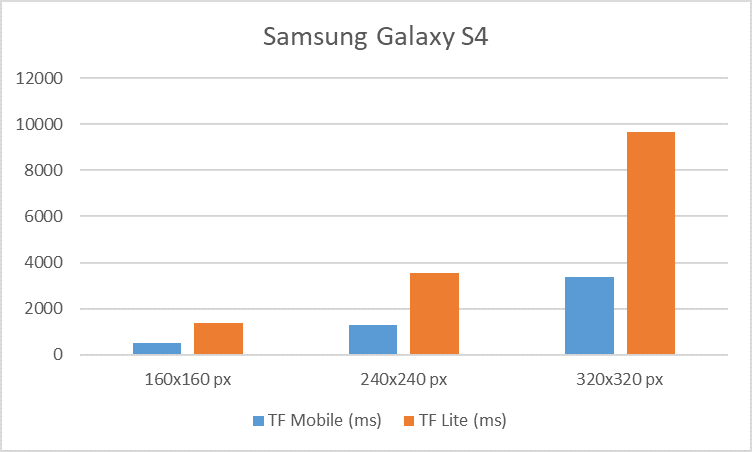
\includegraphics[width=\linewidth]{img/charts/S4.png}
  \captionof{figure}{\small Samsung Galaxy S4 average inference times. This figure reflects the data from table \ref{table:S4}}
  \label{fig:S4}
\end{figure}

\subsection{Test 4: Moto G 5 Plus}
The Moto G 5 Plus belongs to a different family of devices, produced by Motorola. Since its initial release, the Moto G line has always offered middle-class devices with decent specifications at a low price. It is known of Motorola to generally supply its smartphones with the latest OS available, as well as sending regular updates. At the moment of the test, the device was running on Android 7.0, achieving acceptable results and even outperforming the Samsung Galaxy S4 and S5. Table \ref{table:G5} and Figure \ref{fig:G5} reflect the resulted values of processing the collected data with statistics, the data analysis tool selected in the methodology. \\

\begin{table}[h!]
\centering
\resizebox{\textwidth}{!}{%
\begin{tabular}{@{}rcrlrrl@{}}
\toprule
\multicolumn{1}{l}{\textbf{Moto G5 Plus}} & \multicolumn{3}{l}{\textbf{TF Mobile}} & \multicolumn{3}{l}{\textbf{TensorFlow Lite}} \\ \midrule
\multicolumn{1}{|l|}{} & \multicolumn{1}{l}{\textit{$\overline{x}$ (ms)}} & \multicolumn{1}{l}{\textit{$\sigma$ (ms)}} & \multicolumn{1}{l|}{\textit{RSD $\sigma$/ $\overline{x}$ (\%)}} & \multicolumn{1}{l}{\textit{$\overline{x}$ (ms)}} & \multicolumn{1}{l}{\textit{$\sigma$ (ms)}} & \multicolumn{1}{l|}{\textit{RSD $\sigma$/ $\overline{x}$ (\%)}} \\ \cmidrule(l){2-7} 
\multicolumn{1}{|r|}{\textbf{160x160 px}} & \multicolumn{1}{c|}{577,66} & \multicolumn{1}{r|}{8,6} & \multicolumn{1}{l|}{1,5} & \multicolumn{1}{r|}{1148,74} & \multicolumn{1}{r|}{7,2} & \multicolumn{1}{l|}{0,6} \\ \cmidrule(l){2-7} 
\multicolumn{1}{|r|}{\textbf{240x240 px}} & \multicolumn{1}{c|}{1276,94} & \multicolumn{1}{r|}{7,4} & \multicolumn{1}{l|}{0,6} & \multicolumn{1}{r|}{2562,28} & \multicolumn{1}{r|}{18,0} & \multicolumn{1}{l|}{0,7} \\ \cmidrule(l){2-7} 
\multicolumn{1}{|r|}{\textbf{320x320 px}} & \multicolumn{1}{c|}{2259,64} & \multicolumn{1}{r|}{8,7} & \multicolumn{1}{l|}{0,4} & \multicolumn{1}{r|}{4542,26} & \multicolumn{1}{r|}{19,0} & \multicolumn{1}{l|}{0,4} \\ \bottomrule
\end{tabular}%
}
\caption{Moto G5 Plus test results}
\label{table:G5}
\end{table}

\begin{figure}[p]
  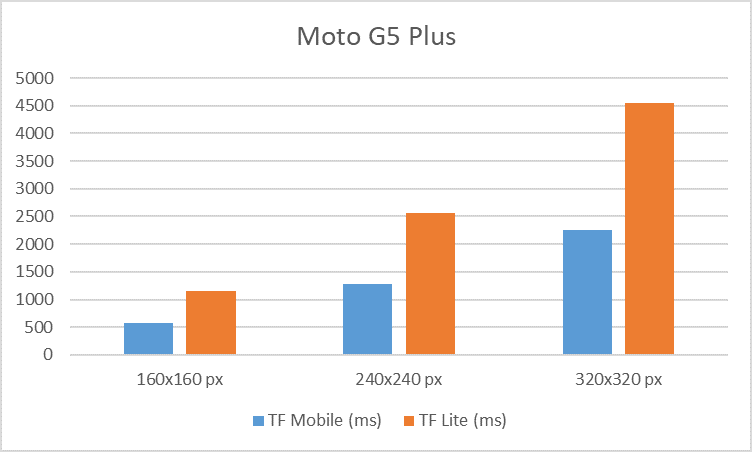
\includegraphics[width=\linewidth]{img/charts/MG5+.png}
  \captionof{figure}{\small Moto G5 Plus . This figure reflects the data from table \ref{table:G5}}
  \label{fig:G5}
\end{figure}

In this section the raw data collected on the experimental tests performed in the four different devices has been thorougly presented. In the next section it will be crunched down and conclusions will be drawn from it. \\

\newpage
\section{Results}
The following section presents the results of the thesis, comparing first the collected and analysed data between the different tests and then interpreting its implications.
\subsection{Comparison of collected data across devices}
As aforementioned, three sets of 50 images, with dimensions $ 160\times160 $, $ 240\times240 $, and $ 320\times320 $ pixels were used to perform the tests. They were created with the credit card image generator that Slagkryssaren provided. The application was compiled and run with each set of images on four different Android devices, namely a Samsung Galaxy S8, a Samsung Galaxy S5, a Samsung Galaxy S4 and a Motorola Moto G5 Plus. The reason to test the models with several image sizes was to check how the inference time grows in relation to the volume of pixels that have to be processed. The processors on the selected devices to run the application represent appropriately the spectrum of processing power in nowaday's mobile phones. Some of them are high class devices whereas others are more outdated. They run as well different versions of the Android operating system. \\

Table \ref{table:averages} presents the average time taken for each model to run over the images of different sizes for each telephone. Surprisingly, the time taken for TensorFlow Lite to run is much longer than TensorFlow Lite. In Table \ref{table:proportions} the proportion between both model's inference time is calculated. In the devices running more recent versions of Android, the proportion stays around 2.0, while in the ones with an older operating system it can go up to 2.9. \\

\begin{table}[h!]
\centering
\resizebox{\textwidth}{!}{%
\begin{tabular}{@{}lrrrrrr@{}}
\toprule
 & \textbf{160x160 px} & \textbf{} & \textbf{240x240 px} & \textbf{} & \textbf{320x320 px} &  \\ \midrule
\multicolumn{1}{|l|}{} & \multicolumn{1}{c|}{TfMobile} & \multicolumn{1}{c|}{TfLite} & \multicolumn{1}{c|}{TfMobile} & \multicolumn{1}{c|}{TfLite} & \multicolumn{1}{c|}{TfMobile} & \multicolumn{1}{c|}{TfLite} \\ \midrule
 \multicolumn{1}{|l|}{\textbf{Moto G 5+}} & 577,66 & 1148,74 & 1276,94 & 2562,28 & 2259,64 & 4542,26 \\ \cmidrule(r){1-1}
\multicolumn{1}{|l|}{\textbf{Samsung S4}} & 516,9 & 1397,58 & 1307,1 & 3562,82 & 3360,74 & 9679,18 \\ \cmidrule(r){1-1}
\multicolumn{1}{|l|}{\textbf{Samsung S5}} & 462,9 & 1006,38 & 931,6 & 2212,34 & 2587,76 & 5777,78 \\ \cmidrule(r){1-1}
\multicolumn{1}{|l|}{\textbf{Samsung S8}} & 182,44 & 371,52 & 410,12 & 814,16 & 757,34 & 1494,28 \\ \bottomrule
\end{tabular}%
}
\caption{\small Average inference time on each device for the three sets of images}
\label{table:averages}
\end{table}

\begin{table}[h!]
\centering
\resizebox{\textwidth}{!}{%
\begin{tabular}{@{}|lcrrr|@{}}
\toprule
 & \multicolumn{1}{l}{\textbf{Android version}} & \multicolumn{1}{l}{\textbf{Ratio 160px}} & \multicolumn{1}{l}{\textbf{Ratio 240px}} & \multicolumn{1}{l|}{\textbf{Ratio 320px}} \\ \midrule
\multicolumn{1}{|l|}{\textbf{Moto G 5+}} & \multicolumn{1}{c|}{\textit{7.0}} & 1,99 & 2,01 & 2,01 \\
\multicolumn{1}{|l|}{\textbf{Samsung S4}} & \multicolumn{1}{c|}{\textit{4.4.2}} & 2,70 & 2,73 & 2,88 \\
\multicolumn{1}{|l|}{\textbf{Samsung S5}} & \multicolumn{1}{c|}{\textit{5.0.1}} & 2,17 & 2,37 & 2,23 \\
\multicolumn{1}{|l|}{\textbf{Samsung S8}} & \multicolumn{1}{c|}{\textit{8.0}} & 2,04 & 1,99 & 1,97 \\ \bottomrule
\end{tabular}%
}
\caption{\small Ratio between TensorFlow Lite and TensorFlow Mobile average inference times.}
\label{table:proportions}
\end{table}

\subsection{Interpretation of results}
The most outstanding result probably is that the TensorFlow Lite model is considerably slower than its counterpart on TensorFlow Mobile. Theoretically, TensorFlow Lite is claimed to be an improved version of its predecessor, built from the ground to be faster and more efficient. However, it has been empirically shown that this is not the case, at least for convolutional neural networks. As has been explained, the TensorFlow library is designed for a wide variety of machine learning graphs, and not only CNNs, so this lack of performance does not necessarily apply to other TensorFlow Lite operations. \\

As stated in the section \ref{sssec:validity} in the methodology to guarantee the validity of the collected data, that the inference time stamps were being correctly measured, the Android Profiler available in Android Studio was used. This tool monitors in real-time the activity of an application, and it helped to reassure that the \textit{tflite.run(inputData, outputData)} function which can be seen in listing \ref{lst:codeTfLite} was really being executed for an unexpected long time. After some research, the conclusion that the TensorFlow Lite library is in an early development stage was made. It was first released in November 2017 \cite{techcrunch}, and even though the engineers at TensorFlow are making great efforts to match the already existing TensorFlow Mobile the library is far from being completed and optimized. When running the app with various releases of TensorFlow Lite which have taken place during the first semester of 2018 substantial differences in its execution time have been found, so the efficiency problems present in the last TensorFlow Lite stable release will probably be solved in the near future. \\

Other interesting results come when contrasting the inference time between devices. Figure \ref{fig:chartTflite} and figure \ref{fig:chartTfMobile} plot the inference time of each device in relation to the amount of work (number of processed pixels) in TensorFlow Lite and Mobile respectively. Firstly, the Samsung Galaxy S8, the device with the most powerful processor, totally overthrows the rest, taking as little as 182 ms to run the TensorFlow Mobile model. A straightforward and obvious conclusion can be drawn: the more processing power a telephone has the faster it will run a TensorFlow model. But not everything depends exclusively on the hardware, the device's software has also an important impact to be considered. This can be seen by comparing the inference time taken by the Samsung Galaxy S5 and the Moto G5 Plus. The former has a better processor with a higher clock speed (2,5 GHz with 4 cores) but runs an older operating system (Android 4.4). With the latter exactly the opposite happens, its processor is not as fast (2,0 GHz with 8 cores) but has Android 7.0 installed. It can be seen in Figures \ref{fig:chartTflite} and \ref{fig:chartTfMobile} how with a smaller workload the Samsung S5 accomplishes lower inference time, but when the size of the image increases the Moto G5 Plus performs better since its software is more prepared. \\

In general, the devices with a more modern operating system suited for these kinds of tasks (Samsung S8 and Moto G5+) prove to have a linear evolution in terms of performance when the image size increases. In contrast, the older devices with a more outdated operating system show to have an exponential evolution of the inference time. They are unable to manage big workloads. A more modern OS allows the device to make measurements which are less disperse (Samsung S8 and Moto G5+ have considerably lower standard deviation than the rest of devices). \\

%\subsection{Conclusions}
After obtaining and analyzing the results of this study in the form of empirical data some conclusions are ready to be drawn. First of all, as aforementioned, convolutional neural networks are not yet optimized for TensorFlow Lite, which makes them run slower than their equivalent in TensorFlow Mobile. This is due to the early development stage in which TensorFlow Lite is at the moment. The second conclusion is that both hardware and software affect the performance of the CNN execution. A more powerful processor will drop the inference time of the network, and a more recent version of Android will handle greater amounts of data with ease, making the execution time grow linearly with the network's workload. In contrast, the inference time increases exponentially with the workload in devices with an older operating system. The reliability of the measurements goes hand in hand with the version of the operating system. It has been show on the Test execution section that the devices running more modern versions of Android (Table \ref{table:S8} and Table \ref{table:G5}) have a lower relative standard deviation than the devices with older operating systems (Table \ref{table:S5} and Table \ref{table:S4}). \\


\begin{figure}[p]
  \includegraphics[width=\linewidth]{img/chartTflite.png}
  \captionof{figure}{\small Performance comparison of TF Lite across devices. The X axis represents the workload (number of pixels). The inference time varies from 371 to 9679 ms.}
  \label{fig:chartTflite}
\end{figure}
\begin{figure}[p]
  \includegraphics[width=\linewidth]{img/chartTfmobile.png}
  \captionof{figure}{\small Performance comparison of TF Mobile across devices. The X axis represents the workload (number of pixels). The inference time varies from 182 to 3360 ms.}
  \label{fig:chartTfMobile}
\end{figure}

\subsection{Project evaluation}
The chosen methodologies and methods are from an overall perspective, suitable to the problem statement and the research done. A sufficiently large dataset is collected in the test running the experiment design. This design fulfils the demanded requirements of validity, reliability, replicability and ethics; so conclusions can be safely drawn from it. The project could have been performed from a different methodological approach, choosing other methods such as case study, for example. This would have presented several differences in the execution of the project, both in the form of advantages and disadvantages. However, the experimental analysis of the TensorFlow frameworks has been successful enough, and even a deliverable (the application itself) was produced, which easily lets other graphs be compared. The software development method Scrum proved to be apropriate and adequately adapted to the situation of one single developer. 
\subsubsection{Feedback from Slagkryssaren}
Slagkryssaren was satisfied with the work done, and also surprised with the obtained results. They consider that this is a topic worth to keep investigating in. They agree that it might be a matter of interest to extend the testing to other devices with different versions of Android in order to get a more accurate idea of the influence that the characteristics of each device has on the results of the test. \\

\newpage
\section{Conclusions and future work}
%Describe the conclusions (reflect on the whole introduction given in Chapter 1). 
%Discuss the positive effects and the drawbacks. 
%Describe the evaluation of the results of the degree project.
%Describe valid future work. 

This thesis presents an analysis of the variation of the execution speed of a convolutional neural network depending on if it is run as a TensorFlow Lite model or as a TensorFlow Mobile model. This was done in collaboration with Slagkryssaren, a software development company based in Stockholm. This company stated a series of requirements for the project and provided with guidance and assistance in its completion. The main focus of the project was to export an specific convolutional network implemented in TensorFlow to the Mobile and Lite versions of the library, for later embedding the resulting models in an Android application and testing it in different devices. The purpose of this thesis, to present the comparison between this two frameworks and the related research done, has been accomplished succesfully in this report. \\

The goal of the project, providing with a solution in the form of an Android application which allows the comparison of the execution speed of a CNN implemented in both TensorFlow Lite and TensorFlow Mobile has been achieved, as well as its subgoals, namely getting acquainted with the TensorFlow framework, exporting the CNN graph in the Lite and Mobile formats, developing the test application in Android and running the tests to compare the two models. The problem statement, which questions how much does TensorFlow Lite improve over its predecessor TensorFlow Mobile, is now answered: there is not yet an improvement in the performance of CNNs but a decay. Through a literature study related work has been conveniently analyzed and the knowledge adquired from it utilized in the thesis. From all the study, the three related works with highest impact in the project are described: a comparative study between TensorFlow and Microsoft CNTK which gave insights about other existing machine learning frameworks; a descriptive report of TensorFlow's performance in large scale systems, which made an impact in the system's architecture design; and the Alexnet paper which helped understanding the design of the CNN. \\

\subsection{Discussion}
The project requirements from the stakeholder together with the system architecture designed were described in detail. These helped to design the system architecture and to put it into realization. Methodological theory was presented at its different levels, with several research methods described. From these, some were chosen giving a motivation and subsequently applied to the research. A deductive approach was selected due to the nature of the problem statement, the experiment was used as data collection method, and statistics as the data analysis method. Also, the interview is punctually used to collect information about the project's requirements from the stakeholders. Regarding software development methods, several approaches were studied to perform this project. To plan the steps of its execution, the agile development method Scrum was utilized. The Android platform was chosen to develop the test application, and Git was the version control system used, together with the Gitflow workflow. \\

This study has several delimitations. The most influential is possibly restricting the performance comparison exclusively between TensorFlow Lite and TensorFlow Mobile, without taking into account other machine learning libraries. Another big delimitation analysing the performance between the two frameworks only in the context of convolutional neural networks, not taking into consideration other kinds of networks. Of course, all conclusions drawn apply only to CNNs. Other delimitations are the small number of devices in which the tests are performed as well as their respective operative systems. With a bigger supply of devices measurements which represent better the general performance of the TensorFlow frameworks could have been made. As well due to time constraints there were few (only 3) image sizes to test the models on each device. A set of images with more continuously distributed sizes would have shown how the ammount of work affects the performance of the models in a more reliabe fashion. \\

\subsection{Future work}
Subsequent future work could be done on this matter, by waiting until a stable and efficient version of TensorFlow Lite is released and making the tests again to confirm that it has performance improvements. As well, other machine learning libraries could be considered in future work, and analyse their performance in relation to the TensorFlow frameworks. During this research, an attempt was made of performing the tests in a Pixel 2 phone, but the tests failed due to technical problems. Tests on this device were of special interest for its capability of using TensorFlow Lite with NNAPI (Android neural networks API) which is designed to run machine learning models. This chip would enormously boost the performance of the CNN running in TensorFlow Lite, and it would be fascinating to test how far can the NNAPI go. Some other possible improvements are enlarging the set of smartphones used for the tests. The selection of devices attempted to cover the whole quality range of Android devices in the market. Nevertheless, it is obvious that this number falls too short to give an accurate insight into the whole spectrum of phones. Another improvement that could have been interesting to do but was not feasible due to time constraints is to check the performance of the TensorFlow models in each device but running on different versions of the operating system. Such a study would have given a clearer idea of how the OS affects the results. This would have meant to manually download and install several versions of the OS for each device, and run the tests on them but it would have taken too much time and it was out of the scope of this project. This is something that could be studied in the future.
